%%%%%%%%%%%%%%%%%%%%%%%%%%%%%%%%%%%%%%%%%%%%%
%INTRODUCTION
%%%%%%%%%%%%%%%%%%%%%%%%%%%%%%%%%%%%%%%%%%%%%
% Strcture
%----------
% - Pathogens spread 
% - Distribution of Foc is prime example 
% - TR4 is a strong reason to monitor the distribution and genetic makeup of Fwb pathogens.
% - Lack of data from world's largest producer and climate change is a threat. 
% - We're sequencing isolates...
%%%%%%%%%%%%%%%%%%%%%%%%%%%%%%%%%%%%%%%%%%%%%

\section{Introduction}

The history of \acf{Focub} exemplifies the profound impact  pathogen spread and diversification can have on global crop production and economies. Although first reported in Australia in 1876 by \textcite{Bancroft1876}, current evidence suggests that the center of origin for \ac{Focub} is Southeast Asia, where it co-evolved with its \textit{Musa} host \parencite{Maryani2019}. Global banana cultivation   inadvertently introduction of \ac{Focub} to new regions, leading to severe damage of banana crops \parencite{Kema2021}.

Notable early dispersion of \acf{Focub1} occurred in South America. First reports in the region came from Panama and Costa Rica in the 1890s, where \ac{Focub1} acquired the common name, Panama disease \parencite{Ashby1913}. From there, \ac{Focub1}  spread across 'Gros Michel' plantations in Jamaica (1903), Suriname (1906), Trinidad and Tobago (1907), Cuba (1908), Guatemala (1910), Colombia (1929), and Venezuela (1930). By the mid 20th century, the banana export industry had been decimated by the \ac{fwb} epidemic. \Ac{Focub1} is now widely distributed in banana producing countries, where it affects many local varieties \parencite{Dita2018}.

Current global production of banana is dominated by the Cavendish variety, which takes its name from William Spencer Cavendish, the sixth duke of Devonshire. Cavendish plants were originally brought to the duke's residence, Chatsworth House, Derbyshire, UK (1829) after their discovery in Southern China in 1826 by British colonial botanists. Shoots from Chatsworth's Cavendish were distributed to British colonies across the globe and resistance to \ac{Focub1} was eventually identified. By the 1950s the banana export industry had substituted the 'Gros Michel' variety for the Cavendish subgroup \parencite{Ploetz2005, Dita2018}. However, in the following decades, Cavendish banana plants in Taiwan were observed displaying symptoms of \ac{Focub} infection \parencite{Agrios2005}. By the 1990s, the same strain of \ac{Focub} was devastating Cavendish plantations in Western Indonesia and peninsular Malaysia \parencite{Kema2021}. 

Identified in 1994 as \ac{Focub} \acf{tr4} \parencite{Ploetz1994}, the race affecting Cavendish bananas has continued to spread. \Ac{Focub4} arrived in China from Taiwan in 1996, later expanding to Laos, Myanmar, and Vietnam. A first report was also recorded for Australia in 1997 \parencite{Ploetz2015a}. In 2005, \ac{Focub4} was recorded in the Philippines, rapidly spreading in Mindanao \parencite{Molina2009}. In the past 15 years, first reports of \ac{Focub4} have been published frequently, with occurrences in Pakistan (2012), Lebanon (2013), Oman (2013), Jordan (2013), Mozambique (2013), India (2015), Israel (2016), Colombia (2019), Peru (2021), and Venezuela (2023) (Figure: \ref{fig:FocDis}) \parencite{Butler2013, Ploetz2015a, Ordonez2015, Zheng2018, Thangavelu2019, Garcia-Bastida2020, Maymon2020, Kema2021, Acuna2022,  Herrera2023}.  The rapid expansion of \ac{Focub} poses a significant threat to global banana production, particularly in Asia, which serves as the centre of diversity for \ac{Focub}. Accurate monitoring of pathogen distribution and genetic diversity across the region is essential.  
\begin{figure}[h!]
  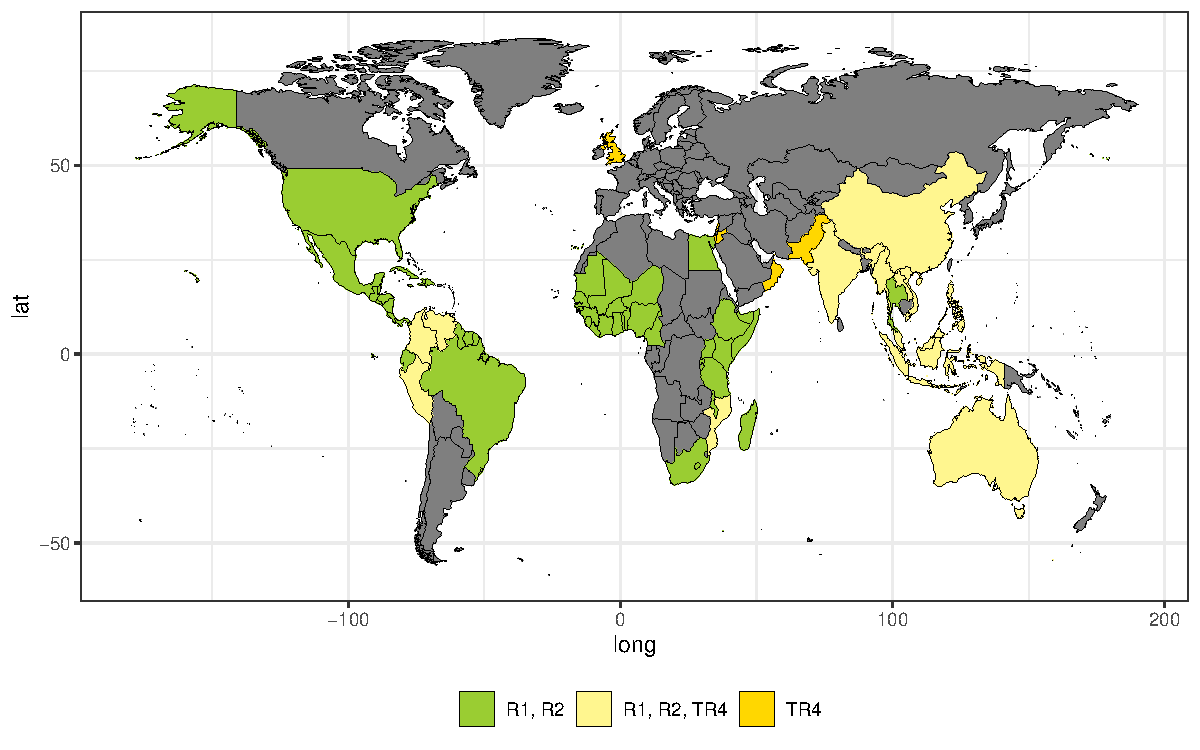
\includegraphics[width=14.5cm]{Figures/FocDis.pdf}
  \caption[Global Distribution of \textit{Fusarium oxysporum} f. sp. \textit{cubense}]{\textbf{Global Distribution of \textit{Fusarium oxysporum} f. sp. \textit{cubense}}. Presence or absence shown by country. Countries which have not reported \ac{Focub} are shown in grey. R1: Race 1, R2: Race 2, TR4: Tropical race 4.}
  \label{fig:FocDis}
\end{figure}

\vbox{
Currently, reports of \ac{Focub4} in India, the top banana-producing country globally, are limited. As the Cavendish cultivar 'Grand Naine' (AAA) accounts for approximately 70\% of India's banana production, \ac{Focub4} is of major concern \parencite{Damodaran2019}.  In 2017, \ac{r1} and R2 (VCG 0124/5 complex) were the dominant races found in India, with reports in the southern states of Andhra Pradesh, Karanata, Kerala, and Tamil Nadu, as well as, Gujarat in the east, and Assam, Nagaland, Uttar Pradesh, and West Bengal in the north-west \parencite{Mostert2017, Thangavelu2020}. Concerningly, in 2019, \textcite{Thangavelu2020} reported some \ac{Focub1} isolates (VCGs 0125 and 01220) caused \ac{fwb} symptoms on the Cavendish cultivar 'Grand Naine' (AAA) in Bihar, Uttar Pradesh, Gujarat, and Tamil Nadu. }

\Ac{Focub4} was first reported in Barari in the state of Bihar in 2015, and has continued to spread; since  reported in Mansahi, Kursela, Falka, Korha, and Pothia in the Katihar district and in Dhamdhaha and Rupoli in the Purnia district \parencite{Thangavelu2019}. \textcite{Viljoen2020} warned that \ac{Focub4} was likely to spread from Bihar to Madhya Pradesh, Maharashtra, and the Uttar Pradesh, as vehicles and labourers frequently move between the states. \ac{Focub4} has now been reported in Kushi Nagar and Ambedkar Nagar in the state of Uttar Pradesh (Figure: \ref{fig:FocDisIndia}) \parencite{Damodaran2019, Thangavelu2019}, but limited data and no biological materials have been provided to identify the strain(s) present \parencite{Kema2021}. As \ac{Focub} spreads through India, necessitating containment measures, the demand for rapid, precise diagnostics and monitoring of pathogen genetic diversity becomes increasingly evident. Particularly given reports of \ac{Focub1} causing disease in Cavendish varieties \parencite{Thangavelu2020}.

\begin{figure}[hp!]
  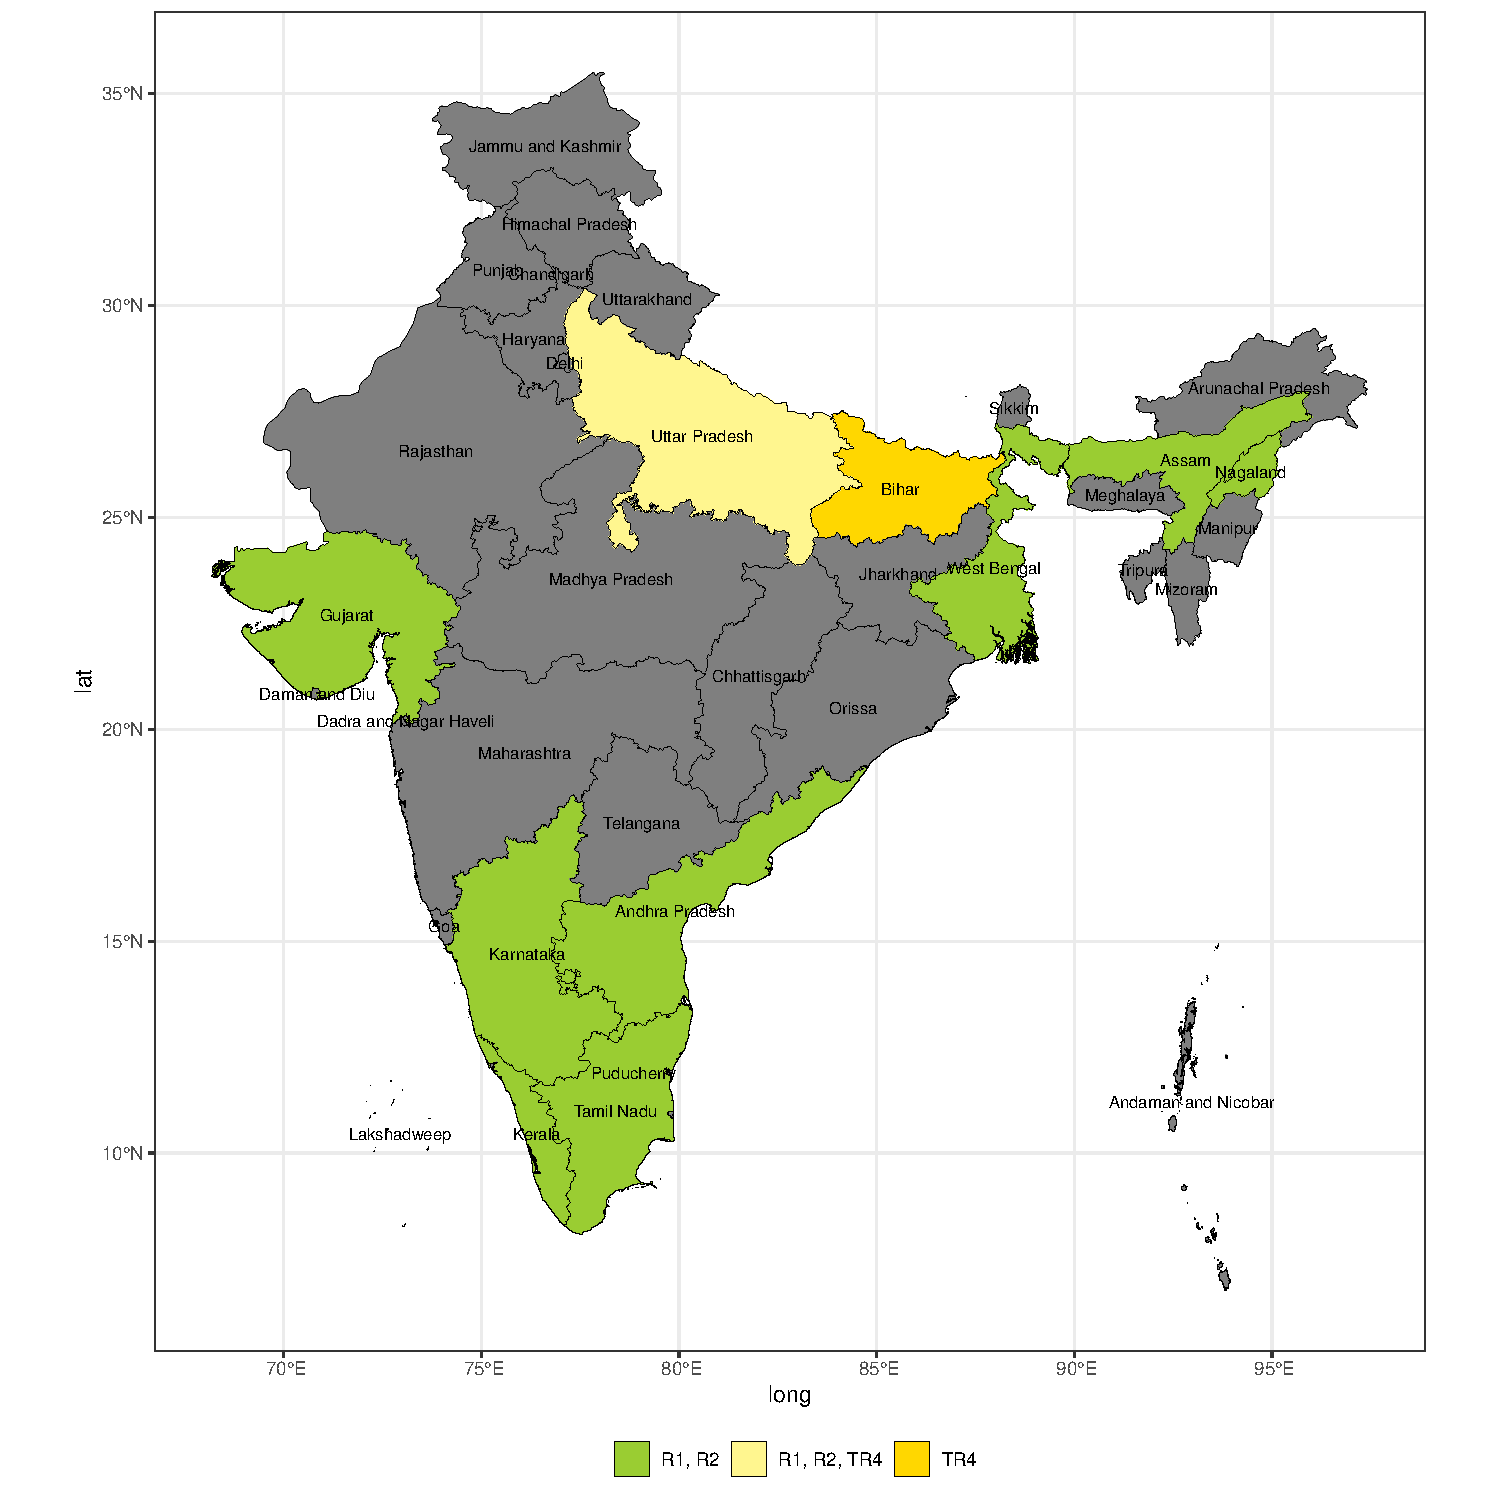
\includegraphics[width=15cm]{Figures/FocDis_India.pdf}
  \caption[Distribution of \textit{Fusarium oxysporum} f. sp. \textit{cubense} in India]{\textbf{ Distribution of \textit{Fusarium oxysporum} f. sp. \textit{cubense} in India}. This map shows presence or absence by states and union territories. Areas which have not reported \ac{Focub} are shown in grey. R1: Race 1, R2: Race 2, TR4: Tropical race 4.}
  \label{fig:FocDisIndia}
\end{figure}

Collaborators at \ac{tnau}, India, assessed \ac{Focub} diversity in Tamil Nadu. Their primary goal was to explore the genetic and molecular underpinnings of banana resistance against \ac{Focub} using advanced next-generation genomics. A survey was conducted in various banana-growing areas of Tamil Nadu to record symptoms of wilt in different banana cultivars. Samples displaying symptoms of \ac{fwb}, including the \ac{Focub4} susceptible Cavendish banana variety 'Grande Naine', were collected from the field, and the pathogen was isolated and cultured in the laboratory. Among the collected samples, isolates SY-2, S6, S16, and S32 were chosen for further analysis. DNA extraction and PCR amplification were performed to confirm the identity of isolates. The isolated strains, S6, S16, and S32, exhibited severe disease symptoms when inoculated into tissue-cultured 'Grand Naine' banana plants and were classified as highly virulent. PCR amplification using race 4-specific primers\footnote{We have been unable to determine which set of primers were used.} confirmed that SY-2, S6, S16, and S32 were \ac{Focub4} isolates, capable of infecting Cavendish banana (Appendix \ref{apx:}).

\vbox{
We generated genome assemblies for the \textit{Fusarium} isolates  (SY-2, S6, S16, and S32) retrieved from Cavendish banana plants and analysed genetic traits. Taxonomic identity and genetic diversity were assessed and suggest that among the strains of \textit{Fusarium} infecting banana in this region are members of a previously unknown species. Of the isolates sequenced, S6 is similar to \ac{Focub} \ac{r1} isolates but displays a \ac{Focub4} phenotype, while SY-2, S16, and S32 belong to the \acf{Ff} species complex. Phylogenetic analysis, read mapping, and \ac{sixg} profiling supported these classifications. It is important to note, however, that bacterial contamination was detected in S6 and S32 isolates, warranting future studies to confirm this potentially novel taxon.}

%%%%%%%%%%%%%%%%%%%%%%%%%%%%%%%%%%%%%%%%%%%%%
%METHODS
%%%%%%%%%%%%%%%%%%%%%%%%%%%%%%%%%%%%%%%%%%%%%
\newpage
\section{Materials and Methods}

\subsection{Analysis of Raw Read data from TNAU isolates}

The raw Illumina paired-end genomic reads for the \textit{Fusarium} isolates SY-2, S6, S16, and S32 were supplied by collaborators at \ac{tnau}\footnote{\textcolor{red}{Due to communication challenges with collaborators at TNAU, we have not been able to establish the extraction protocol used to produce the DNA used for sequencing.}}. Isolates S6, S16 and S32 were reported to be  highly virulent on Cavendish banana. Following FastQC (v0.11.8)
\parencite{Andrews2010} analysis, raw reads were mapped to \ac{Focub4} UK0001 (\href{https://www.ncbi.nlm.nih.gov/datasets/genome/GCA_007994515.1/}{GCA\_007994515.1}) \parencite{Warmington2019} reference genome using Bowtie2 (v2.4.5) \parencite{Langmead2012} (for full command-line arguments and shells scripts see: \href{https://github.com/JamiePike/NewTools-Project/blob/master/docs/Assembly/AssemblyNotes.md}{GitHub Repository}). Due to poor mapping rates for some isolates, 1000 raw reads were examined  from each \ac{tnau} isolate in an attempt to diagnose the issue; they were used as queries in  \ac{ncbi} \href{https://blast.ncbi.nlm.nih.gov/Blast.cgi?PROGRAM=blastn&BLAST_SPEC=GeoBlast&PAGE_TYPE=BlastSearch}{BLASTN searches} against the nr/nt database \parencite{Nih2014}. Raw reads from each isolate were also mapped to high-quality assemblies of the \ac{Focub1} isolate 160527 (\href{https://www.ncbi.nlm.nih.gov/datasets/genome/GCA_005930515.1/}{GCA\_005930515.1}) \parencite{Asai2019} and the \ac{Fs} isolate FS66 (\href{https://www.ncbi.nlm.nih.gov/datasets/genome/GCA_017165645.1/}{GCA\_017165645.1}), reported to cause leaf blight in Cavendish banana \parencite{Cui2021}. Isolates S6, S16 and S32 were also mapped to a reference quality \textit{Stenotrophomonas maltophilia} genome assembly, isolate NCTC10258 (\href{https://www.ncbi.nlm.nih.gov/datasets/genome/GCF_900475405.1/}{GCA\_900475405.1}). 

\subsection{Genome Assembly and Annotation}

\subsubsection{\textit{De novo Assembly}}
A \textit{de novo} assembly was generated for each of the \ac{tnau} isolates using SPAdes (v3.14.1) \parencite{Prjibelski2020} following FastQC (v0.11.8) analysis. SPAdes is routinely used for \textit{Fusarium} genome assembly
(see: \textcite{Armitage2018, Hudson2020, Tanaka2022}). A custom Python script was developed to remove sequences with <25\% GC content from the assembly (see: \href{https://github.com/JamiePike/NewTools-Project/blob/master/bin/gcTrimmer.py}{GitHub}). As raw read data for isolates S6 and S32 contained high levels of contamination, \textit{de novo} assemblies were generated using only reads mapping to reference genomes \ac{Focub1} isolate 160527 (\href{https://www.ncbi.nlm.nih.gov/datasets/genome/GCA_005930515.1/}{GCA\_005930515.1}) \parencite{Asai2019} and \ac{Fs} isolate FS66 (\href{https://www.ncbi.nlm.nih.gov/datasets/genome/GCA_017165645.1/}{GCA\_017165645.1}) \parencite{Cui2021}, respectively. Mapped reads were determined using Bowtie2 (v2.4.5) and were extracted into separate FASTQ files using SAMtools (v1.6, using htslib v1.6) \parencite{Danecek2021}. 

\subsubsection{Contamination Analysis and Quality Assessments}
BlobTools (v1.1.1) \parencite{Laetsch2017} was used for the taxonomic partitioning of the assemblies. The \ac{tnau} assemblies were searched against the \ac{ncbi} nt/nr database using BLASTN (v2.9.0+) and the paired-end raw reads were aligned to each of the assemblies using Bowtie2 (v2.4.5). Taxonomic hits were ranked at the species level using default BolbTools (v1.1.1) settings. To extract contigs that were assigned to a non-\textit{Fusarium} genus by BlobTools (v1.1.1), the output JSON file was filtered using blobtools view, with the -r species flag. Contigs assigned to a \textit{Fusarium} species or "no-hit" were then extracted and saved in a separate text file. The BlobTools (v1.1.1) seqfilter command with the default settings was then used to extract contigs which were assigned to \textit{Fusarium} or had "no-hit".

The quality and completeness of the assembled, contaminant-filtered genomes was estimated using \ac{busco} (v5.4.6) with the hypocreales\_odb10 data set \parencite{Manni2021}. All of the raw reads were mapped back to the assemblies using Bowtie2 (v2.4.5) and a Qualimap (v2.2.2) assessment was conducted \parencite{Garcia-Alcalde2012}. Quast (v5.0.2) \parencite{Gurevich2013}  and gfastats (v1.3.6) \parencite{Formenti2022} were used to generate assembly quality statistics. 

\subsubsection{Identification of Repetitive Elements}

Repetitive elements were identified in each contaminant-filtered assembly using RepeatModeler (v2.0.4) \parencite{Flynn2020} including the -LTRStruct option. Once models had been generated, assemblies were masked iteratively with RepeatMasker (v4.1.5) \parencite{Smit2010} using the ouptut from each round  as input for the following masking step. First small, simple repeats were masked using the -noint and -xsmall options; then assemblies were masked using the default RepeatMasker (v4.1.5)  database (Dfam v3.3) \parencite{Storer2021} using the -species Fusarium option; followed by masking using the models generated by RepeatModeler (v2.0.4).

\subsubsection{Genome Annotation}
Following masking, the \ac{tnau} genomes were annotated using the MAKER pipeline (v3.01.04) \parencite{Holt2011}, including AUGUSTUS (v3.3) \parencite{Stanke2006} for \textit{ab initio} gene prediction with the “Fusarium” species option. As no RNA sequencing data were available for these isolates, homology evidence from a reference set of 387,728 proteins, from the \ac{ncbi} RefSeq nr database \parencite{Agarwala2016}, generated using the search term "Fusarium AND srcdb\_refseq[PROP]", was used. 

\subsection{Phylogenetic Analysis of \ac{tnau} isolates}\label{chap2:phylogeny}

The common \textit{Fusarium} genetic barcodes \ac{tef} and \ac{rbp2} were used to generate phylogenies \parencite{Edel-Hermann2019}. A \ac{tef} and \ac{rbp2} sequence databases were compiled using available reference sequences from the \ac{ncbi} database (Appendix; \ref{apx:}). Homologues of \ac{tef} and \ac{rbp2} were identified in each of our \ac{Fo} assemblies (See section:~\ref{chap3:fusariumdb}) using BLASTN (v 2.9.0+)(1e\textsuperscript{-6} cut-off). The locations of hits with greater than 70\% identity and 90\% coverage were recorded, and the sequence within this region was manually examined and extracted using SAMtools (v1.15.1). The \ac{tef} and \ac{rbp2} regions from each genome were concatenated into a single FASTA file for each barcode. MAFFT (v7.505) \parencite{Katoh2019} was used to construct a multiple sequence alignment, adjusting the direction according to the first sequence to ensure correct alignment and any overhanging regions were trimmed manually. IQ-TREE2 (v2.2.0.3) \parencite{Nguyen2015} was used to infer a maximum-likelihood phylogeny using the ultrafast bootstrap setting for 1000 bootstrap replicates and was visualised using iTOL \parencite{Letunic2021}. Additionally, the extracted \ac{tef} and \ac{rbp2} regions for the \ac{tnau} isolates were searched against the \ac{ncbi} nr/nt database using the  \ac{ncbi} \href{https://blast.ncbi.nlm.nih.gov/Blast.cgi?PROGRAM=blastn&BLAST_SPEC=GeoBlast&PAGE_TYPE=BlastSearch}{BLASTN suite} \parencite{Nih2014}, and the \href{https://fusarium.mycobank.org/page/Fusarium_table}{MycoBank database} \parencite{Robert2013}. 

\subsection{Identification of pathogen-specific features.}

\subsubsection{\textit{Secreted In Xylem} gene identification and phylogenetic analysis}
\label{chap1:tnauSIXgenePhylo}
To identify known \acs{Fo} effectors in the \ac{tnau} assemblies and compare the \ac{sixg} profile to other \textit{Fusaria}, reference sequences for SIX1-SIX14 used by \textcite{Czislowski2018} were downloaded from  GenBank and homologues of each \textit{SIX} gene was identified using TBLASTN (v2.9.0+) (1e\textsuperscript{6} cut-off) in the \ac{tnau} assemblies, as well as publicly available assemblies of \ac{Focub} (n=14), \ac{Fs} (n=2), the \ac{Fo} endophyte Fo47, \ac{Fo} formae speciales \textit{cepae, conglutinans, coriandrii, lini, lycopersici,  rapae} and \textit{vasinfectum}, and \textit{F. graminearum}, which were downloaded from \href{https://www.ncbi.nlm.nih.gov/data-hub/genome/}{GenBank} following a genome search. (Supplementary table x: Genomes table). A binary data matrix indicating presence (“1”) or absence (“0”) was generated using the TBLASTN hit data for visualisation. 

Homologues of each \ac{sixg} identified were extracted for phylogenetic analysis.  The locations of hits were recorded, and the sequence within this region was manually examined and extracted using SAMtools (v1.15.1). Sequences from each genome were concatenated into a single FASTA file for each \ac{sixg} and aligned with  MAFFT (v7.505) \parencite{Katoh2019}, adjusting the direction according to the first sequence to ensure correct alignment. Overhanging regions were trimmed manually. IQ-TREE2 (v2.2.0.3) \parencite{Nguyen2015} was used to infer a maximum-likelihood phylogeny using the ultrafast bootstrap setting for 1000 bootstrap replicates and phylogenies were visualised using iTOL \parencite{Letunic2021}.

\subsubsection{Identification of putative effectors}

To identify \acp{ce} in the \ac{tnau} isolates, the predicted protein set for each isolate was filtered by size (>30aa and <450aa) and submitted to SignalP (v5.0b) \parencite{Petersen2011}. Sequences that were predicted to contain a signal peptide were passed to EffectorP (v2.0.1) \parencite{Sperschneider2018} for effector prediction. The \ac{ce} sets from each genome were then combined and clustered using CD-HIT (v4.8.1) \parencite{Fu2012} at 80\% to identify shared \acp{ce}. 

%\subsubsection{Reference genome alignment and raw read mapping}

%Pathogenicity chromosomes are common among plant pathogenic \ac{Fo} \parencite{Ma2010, Fokkens2020}. As the \ac{tnau} isolate assemblies were too fragmented to characterise  pathogenic regions, \acp{mimp}, \acp{sixg}, and \acp{ce} identified using the Maei pipeline (Chapter \ref{Chap3}) were recorded in the high-quality \ac{Focub4} UK0001 and \ac{Fs} FS66 assemblies, and \ac{tnau} isolate raw reads mapped on to these assemblies using Bowtie2 (v2.4.5). Nucmer (-max match, deltafilter –g) from MUMmer (v4.0.0rc1) \parencite{Marcais2018} was used to align the ac{Focub4} UK0001 and \ac{Fs} FS66 assemblies to identify shared putative pathogenic regions between the assemblies. Circos (v0.69-8) \parencite{Krzywinski2009} was used to visualise virulence factor location and genome alignments. 

\subsection{Data and software availability}

The full computational pipelines, command-line arguments as well as bash, R, and Python scripts used for all analysis outlined are available in the \href{https://github.com/JamiePike/NewTools-Project}{NewTools-Project} GitHub Repository at https://github.com/JamiePike/NewTools-Project, with supporting documentation provided in Markdown format for \href{https://github.com/JamiePike/NewTools-Project/blob/master/docs/Assembly/AssemblyNotes.md}{genome assemblies}, \href{https://github.com/JamiePike/NewTools-Project/blob/master/docs/Annotations/RepeatMaskingNotes.md}{masking repeat elements}, \href{https://github.com/JamiePike/NewTools-Project/blob/master/docs/Annotations/Annotations.md}{annotations}, \href{https://github.com/JamiePike/NewTools-Project/blob/master/docs/Effectors/PredicitionofCandidateEffectors.md}{\ac{ce} identification}, and \href{https://github.com/JamiePike/NewTools-Project/blob/master/docs/Phylogeny/Phylogenies.md}{phylogenetic analysis}.

%%%%%%%%%%%%%%%%%%%%%%%%%%%%%%%%%%%%%%%%%%%%%
%RESULTS
%%%%%%%%%%%%%%%%%%%%%%%%%%%%%%%%%%%%%%%%%%%%%
\newpage
\section{Results}

\subsection{Analysis of Raw Read data from TNAU isolates}

Mapping rates of the raw reads from isolates S6, S16, S32, and SY-2 to the \ac{Focub4} UK0001 assembly (\href{https://www.ncbi.nlm.nih.gov/datasets/genome/GCA_007994515.1/}{GCA\_007994515.1}) were 8.72\%, 53.81\%, 15.69\%, and a 54.11\%, respectively (Table ~\ref{tab:RawReadMapping}). Raw reads from each isolate were also mapped to the \ac{Focub1} 160527 assembly (\href{https://www.ncbi.nlm.nih.gov/datasets/genome/GCA_005930515.1/}{GCA\_005930515.1}), with alignment rates for all \textless 55\%. Due to the low alignment rates, unmapped reads were extracted and a random subset of 1000 reads per isolate was searched using \ac{ncbi} \href{https://blast.ncbi.nlm.nih.gov/Blast.cgi?PROGRAM=blastn&BLAST_SPEC=GeoBlast&PAGE_TYPE=BlastSearch}{web BLASTN suite} \parencite{Nih2014}, which revealed that many of the unmapped reads from these isolates were similar ($\geq90\% $ identity) to sequences from species within \ac{FFSC}. Further, isolates S6 and S32 displayed signs of possible bacterial contamination, with raw reads displaying ($ \geq90\% $ identity) to sequences from \textit{Stenotrophomonas} species, particularly \textit{S. maltophilia}. 

All raw reads from isolates S6, S16, S32, and SY-2 were mapped to a \acf{Fs} reference assembly, isolate FS66 (\href{https://www.ncbi.nlm.nih.gov/datasets/genome/GCA_017165645.1/}{GCA\_017165645.1}). \ac{Fs} is a member of the \ac{FFSC} and FS66 has been reported to cause leaf blight symptoms in banana \parencite{Cui2021}. Raw reads from isolates S6 and S32 had a 5.24\% and 22.49\% mapping rate to the \ac{Fs} reference, respectively, whereas 68.65\% of the raw reads from isolate S16 and 93.96\% of the raw reads from the SY-2 isolate mapped to the \ac{Fs} reference assembly (Table ~\ref{tab:RawReadMapping}). Isolates S6, S16 and S32 were also mapped to a reference-quality \textit{S. maltophilia} genome assembly (\href{https://www.ncbi.nlm.nih.gov/datasets/genome/GCF_900475405.1/}{GCA\_900475405.1}, isolate NCTC10258). Approximately 50\% of raw reads from isolates S6 and S32 mapped to the \textit{S. maltophilia} reference, whereas raw reads from isolate S16 only had a 0.01\% mapping rate to the \textit{S. maltophilia} reference. Further, the raw S6 and S32 reads show a similar GC\% to the \textit{S. maltophilia} reference genome (S6=63\%, S32=61\%, NCTC10258=66.5\%).

\bigskip
% Please add the following required packages to your document preamble:
% \usepackage{booktabs}
% \usepackage{multirow}
% \usepackage{graphicx}
\begin{table}[h!]
\caption[Overall alignment rate of all raw reads from each TNAU isolates to fungal and bacterial reference species]{{\textbf{Overall alignment rate of all raw reads from each TNAU isolates to fungal and bacterial reference species.}} Overall alignment rate determined by Bowtie2 (version 2.4.5). Reference assemblies were downloaded from GenBank: \ac{Focub4} isolate UK0001 (\href{https://www.ncbi.nlm.nih.gov/datasets/genome/GCA_007994515.1/}{GCA\_007994515.1}), \ac{Focub1} isolate 160527 (\href{https://www.ncbi.nlm.nih.gov/datasets/genome/GCA_005930515.1/}{GCA\_005930515.1}), \textit{Fusairum sacchari} isolate FS66 (\href{https://www.ncbi.nlm.nih.gov/datasets/genome/GCA_017165645.1/}{GCA\_017165645.1}), \textit{Stenotrophomonas maltophilia} isolate NCTC10258 (\href{https://www.ncbi.nlm.nih.gov/datasets/genome/GCF_900475405.1/}{GCA\_900475405.1}).}
\label{tab:RawReadMapping}
\centering
\resizebox{\textwidth}{!}{%
\begin{tabular}{cccccc}
\hline
\multirow{2}{*}{\textbf{Reference Species}} & \multirow{2}{*}{\textbf{Strain}} & \multicolumn{4}{c}{\textbf{BOWTIE2 Alignment Rate}} \\ \cline{3-6} 
 &  & \textbf{S6} & \textbf{S16} & \textbf{S32} & \textbf{SY-2} \\ \cline{1-2}
\textit{Fo.} f. sp. \textit{cubense} (TR4) & UK0001 & 8.72\% & 53.81\% & 15.69\% & 54.11\% \\
\textit{Fo.} f. sp. \textit{cubense} (R1) & 160527 & 9.90\% & 53.67\% & 15.51\% & 54.02\% \\
\textit{F. sacchari} & FS66 & 5.24\% & 68.65\% & 22.49\% & 93.96\% \\
\textit{Stenotrophomonas maltophilia} & NCTC10258 & 49.32\% & 0.01\% & 53.93\% & -- \\ \hline
\end{tabular}%
}
\end{table}

\subsection{Contamination Analysis and \textit{de novo} Genome Assembly}

As <55\% of raw reads from the \ac{tnau} isolates aligned to the \ac{Focub1} and \ac{Focub4} reference assemblies, the \ac{tnau} genomes were assembled \textit{de novo}. All raw reads were used for the S16 and SY-2 genome assemblies, and S6 and S32 \textit{de novo} genome assemblies were generated using only reads aligning to the reference genomes \ac{Focub1} isolate 160527 (\href{https://www.ncbi.nlm.nih.gov/datasets/genome/GCA_005930515.1/}{GCA\_005930515.1}) \parencite{Asai2019} and \ac{Fs} isolate FS66 (\href{https://www.ncbi.nlm.nih.gov/datasets/genome/GCA_017165645.1/}{GCA\_017165645.1}) \parencite{Cui2021}, respectively. Following assembly, low-GC contigs  (\textless 25\%) were removed from the SY-2 and S16 assemblies, reducing the total number of contigs from 1,548 to 441 in the SY-2 assembly and 1,666 to 768 in the S16 assembly.  

A BlobTools (v1.1.1) analysis was used to identify any potential contaminant contigs. Although \textit{Fusarium} species accounted for the majority of the \ac{ncbi} nt database hits for the SY-2 genome assembly, with 365 contigs assigned to \ac{Ff}, some potential contamination from \textit{Musa} species was identified, with 14 contigs assigned to \textit{Musa balbisiana} and one assigned to \textit{Musa textilis} (Figure \ref{fig:SY-2:BlobTools}). The S6, S16, and S32 genome assemblies contained hits from only \textit{Fusarium} species or had no species allocated (no-hit) and no other genera were identified. For S16 and S32, the majority of contigs were assigned to \ac{Ff} (Figure \ref{fig:S16:BlobTools}, \ref{fig:S32:BlobTools}), whereas the  S6 genome assembly contained contigs assigned to \ac{Ff} and \ac{Fo}, although 2,301 contigs had no hits (Figure \ref{fig:S6:BlobTools}).  

%%%%%%%%%%%%%%%%%%%%%%%%%%
%%%%% SY-2 BlobTools %%%%%
%%%%%%%%%%%%%%%%%%%%%%%%%%
\begin{figure}[hp!]
    \centering
    \begin{subfigure}[]{0.9\textwidth}
        \centering
        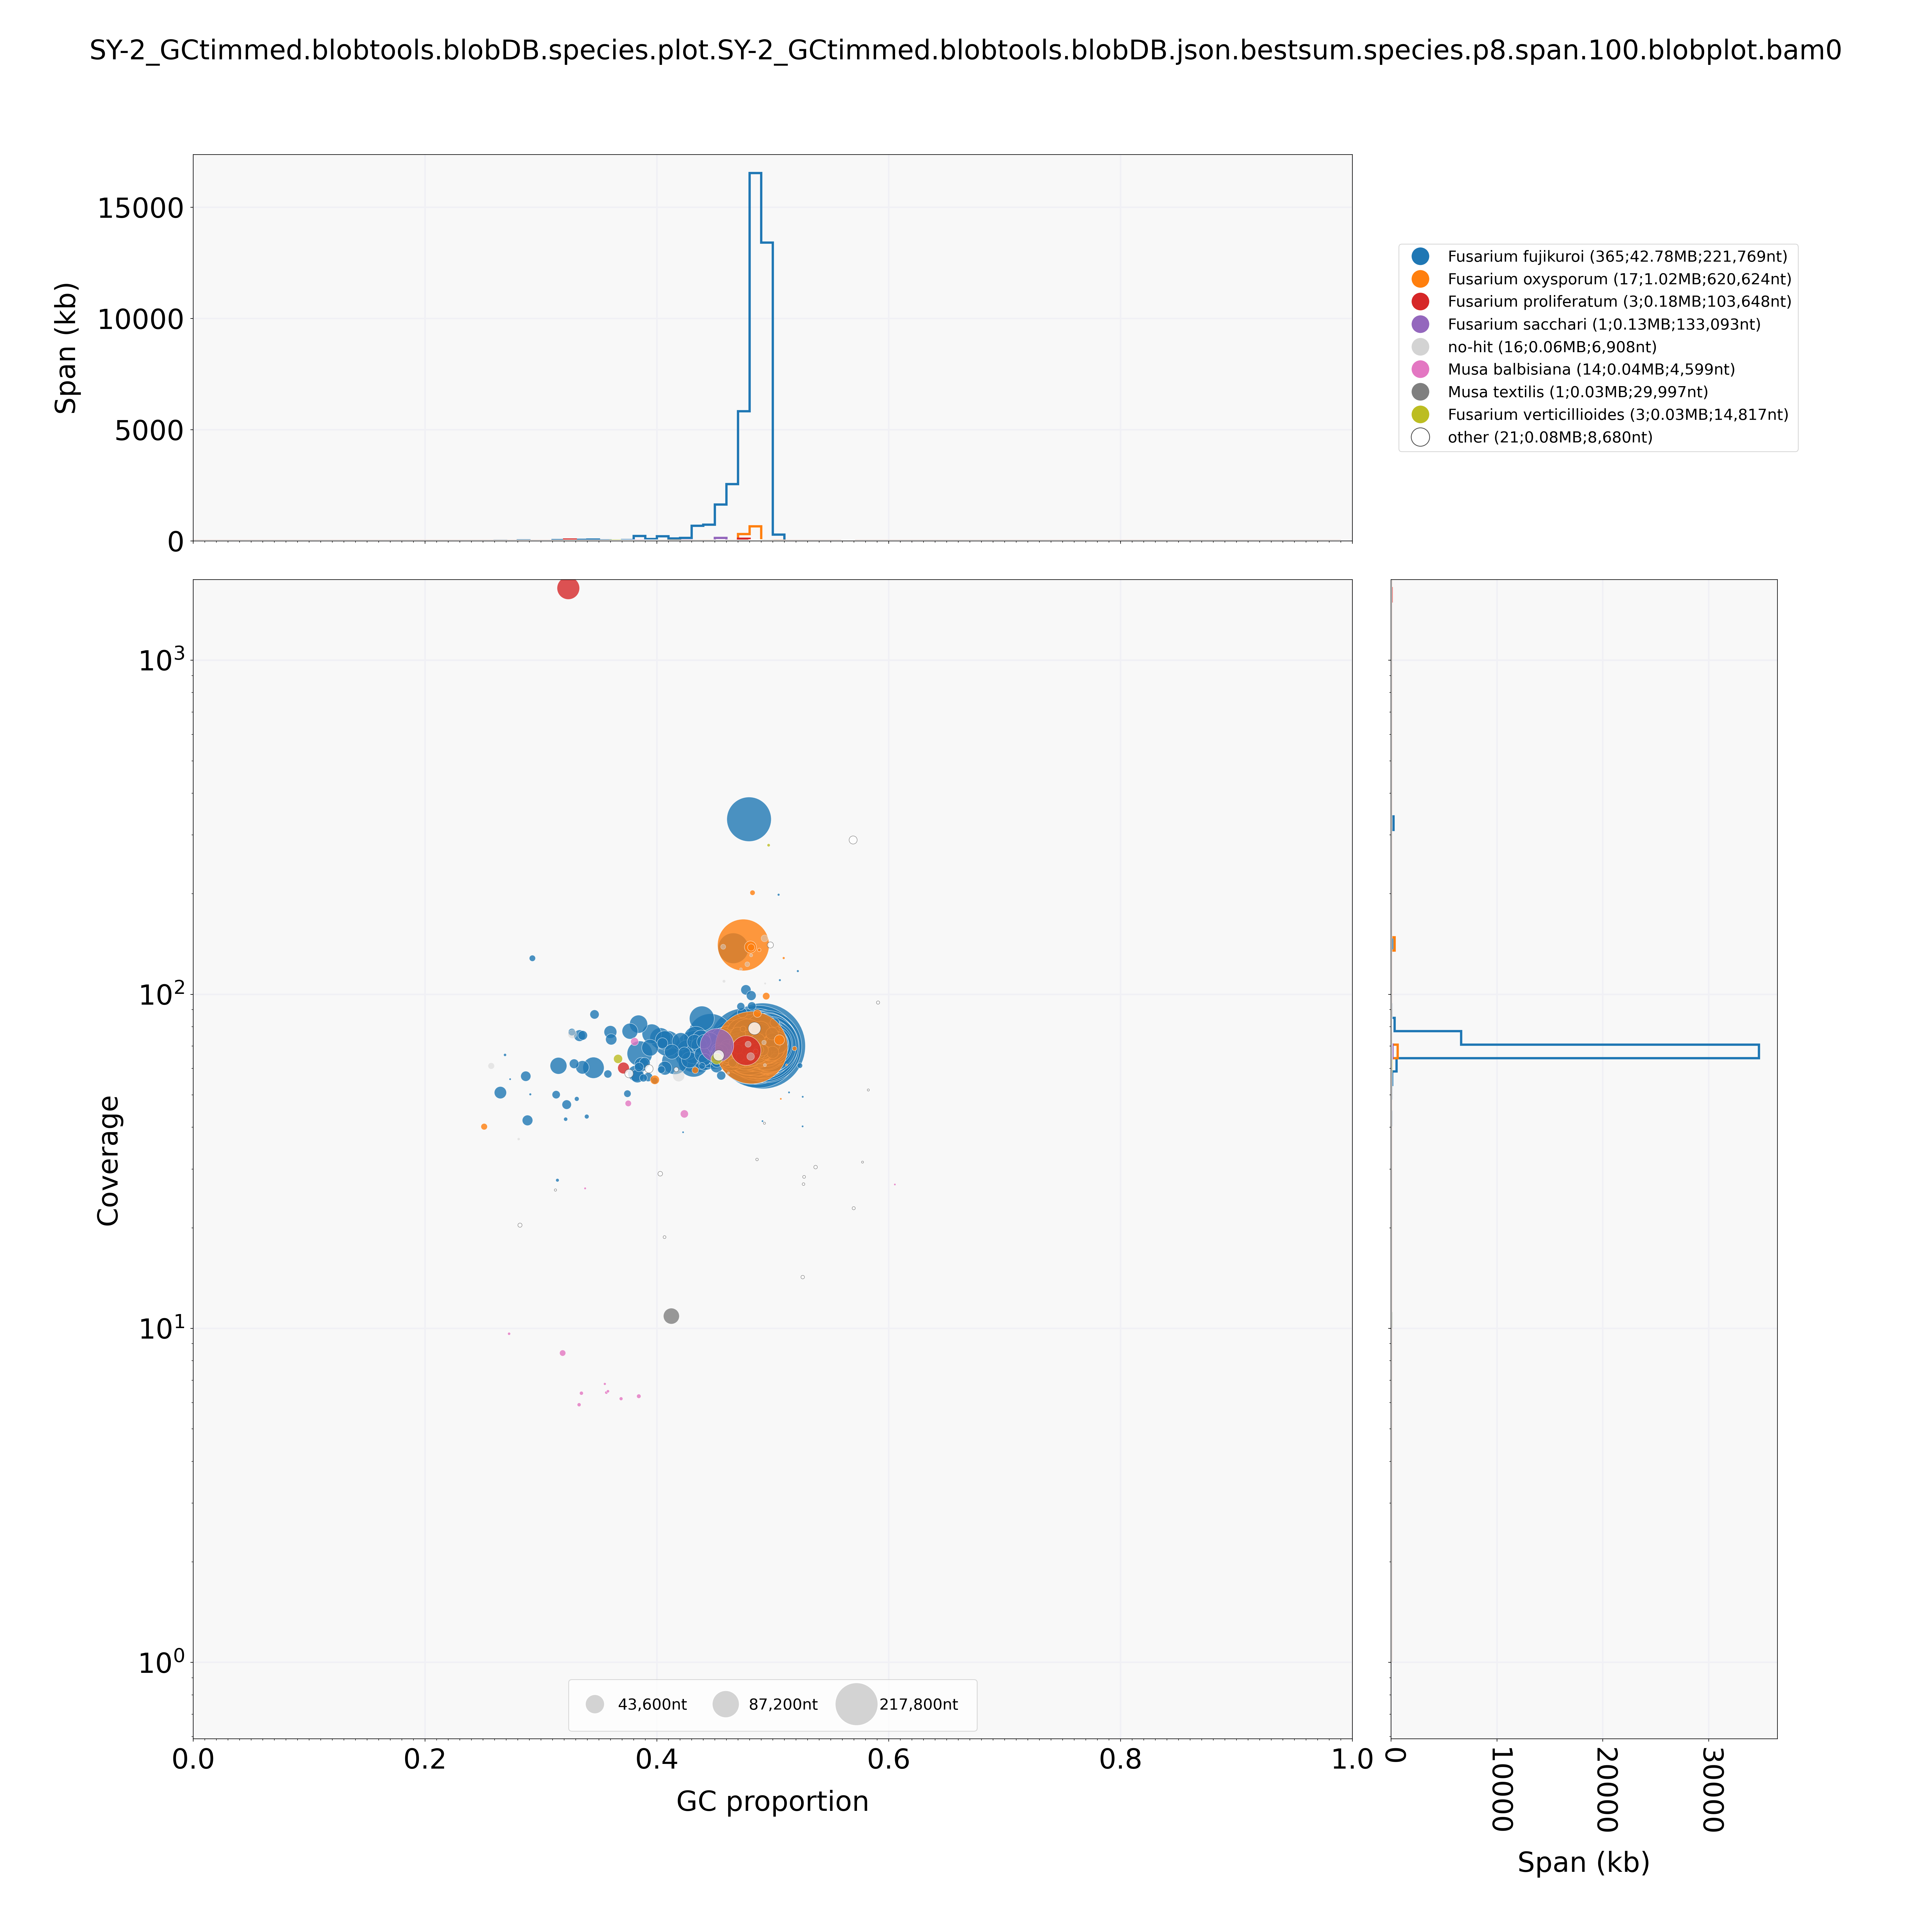
\includegraphics[width=\textwidth]{Appendices/SY-2_GCtimmed.blobtools.blobDB.species.plot.SY-2_GCtimmed.blobtools.blobDB.json.bestsum.species.p8.span.100.blobplot.bam0.png}
        \caption{}
        \label{fig:BlobPlot-SY-2}
    \end{subfigure}
    \begin{subfigure}[]{0.9\textwidth}
        \centering
        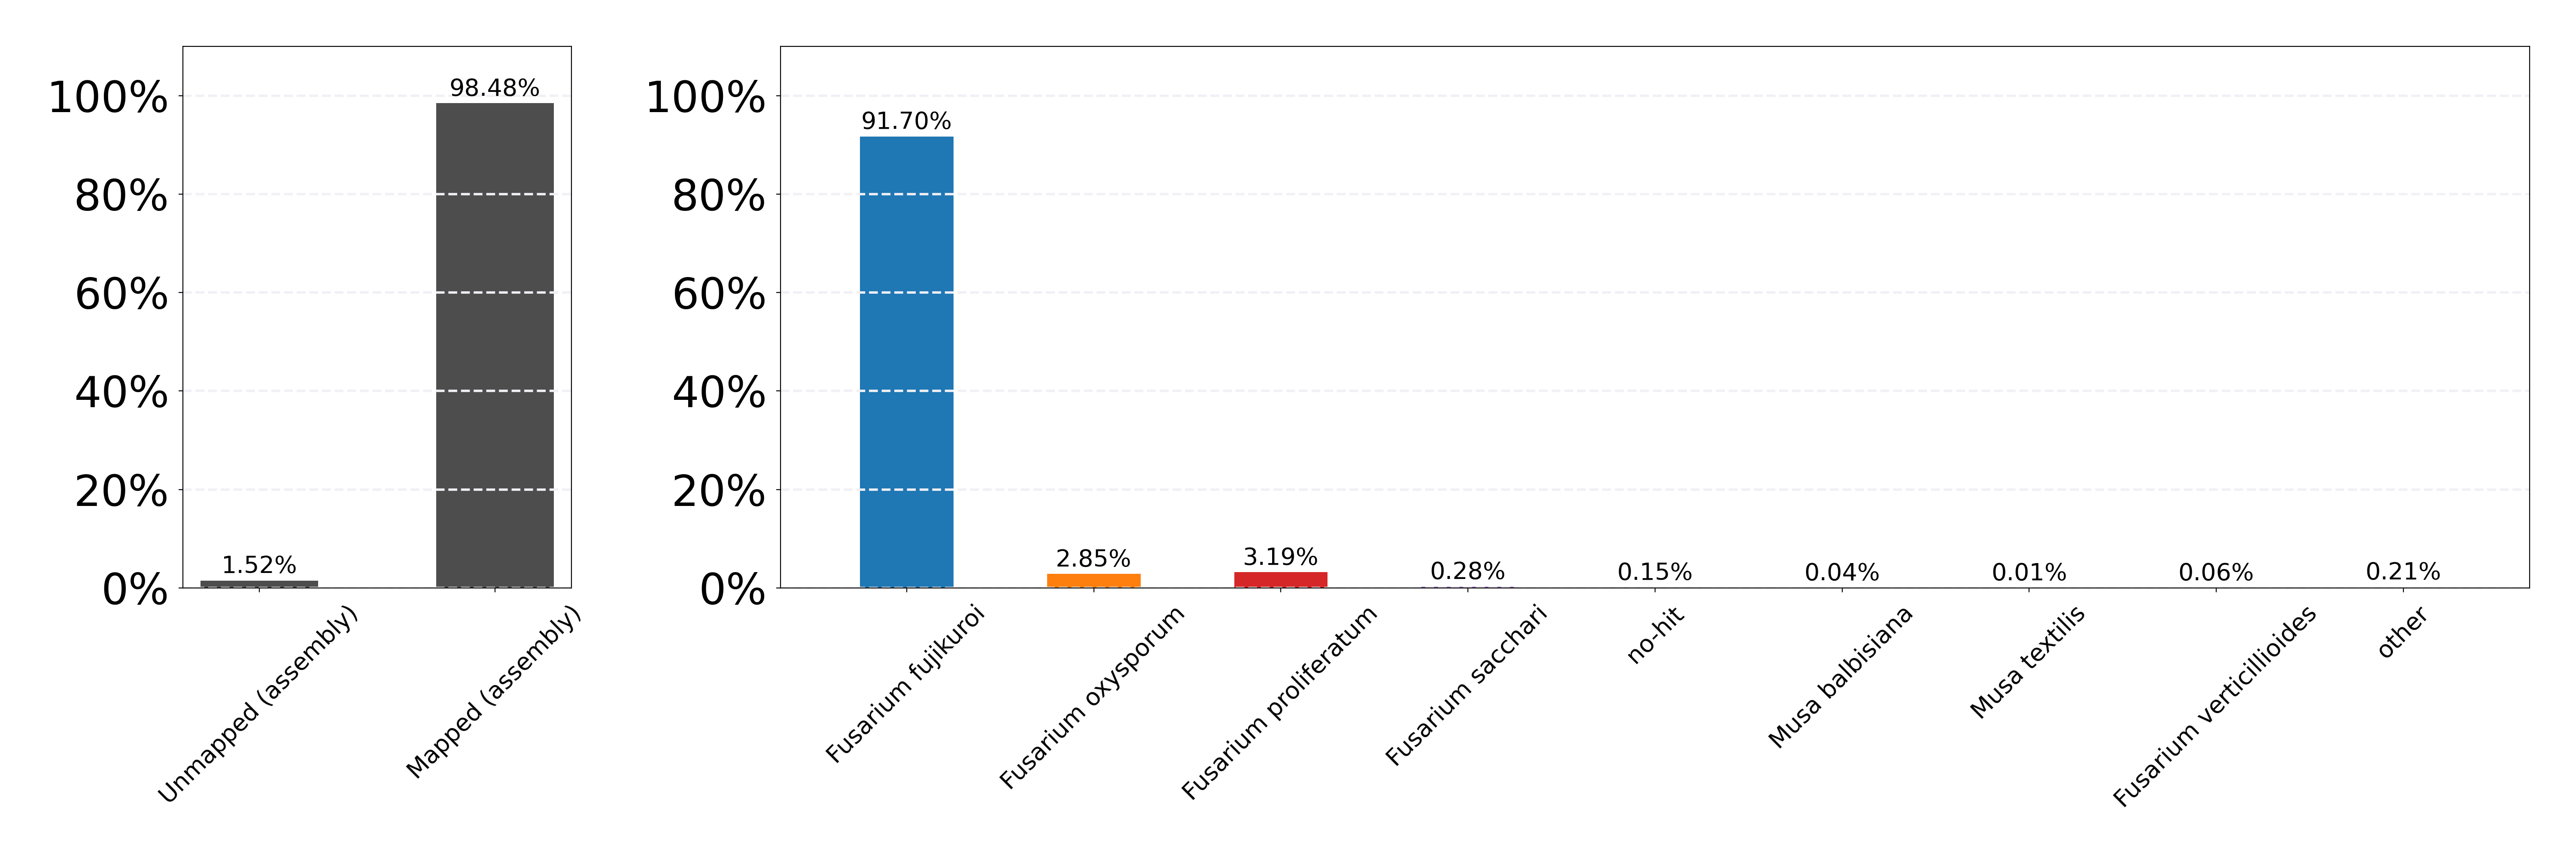
\includegraphics[width=\textwidth]{Appendices/SY-2_GCtimmed.blobtools.blobDB.species.plot.SY-2_GCtimmed.blobtools.blobDB.json.bestsum.species.p8.span.100.blobplot.read_cov.bam0.png}
        \caption{}
        \label{fig:BlobPlot_readcov-SY-2}
    \end{subfigure}
    \caption[BlobTools visualisations of the SY-2 assembly]{\textbf{BlobTools visualisations of the SY-2 assembly shows \acf{Ff} is the most common species hit.}
        \subref{fig:BlobPlot-SY-2} BlobPlot of SY-2. Sequences in the assembly are depicted as circles, with diameter proportional to sequence length and coloured by taxonomic annotation based on BLASTN (v2.9.0+) of NCBI nt database.
        \subref{fig:BlobPlot_readcov-SY-2} Read coverage plot of the SY-2 assembly. Mapped reads are shown by taxonomic group at the rank of species.}
        \label{fig:SY-2:BlobTools}
\end{figure}

%%%%%%%%%%%%%%%%%%%%%%%%%%
%%%%% S16 BlobTools %%%%%%
%%%%%%%%%%%%%%%%%%%%%%%%%%
\begin{figure}[hp!]
    \centering
    \begin{subfigure}[]{0.9\textwidth}
        \centering
        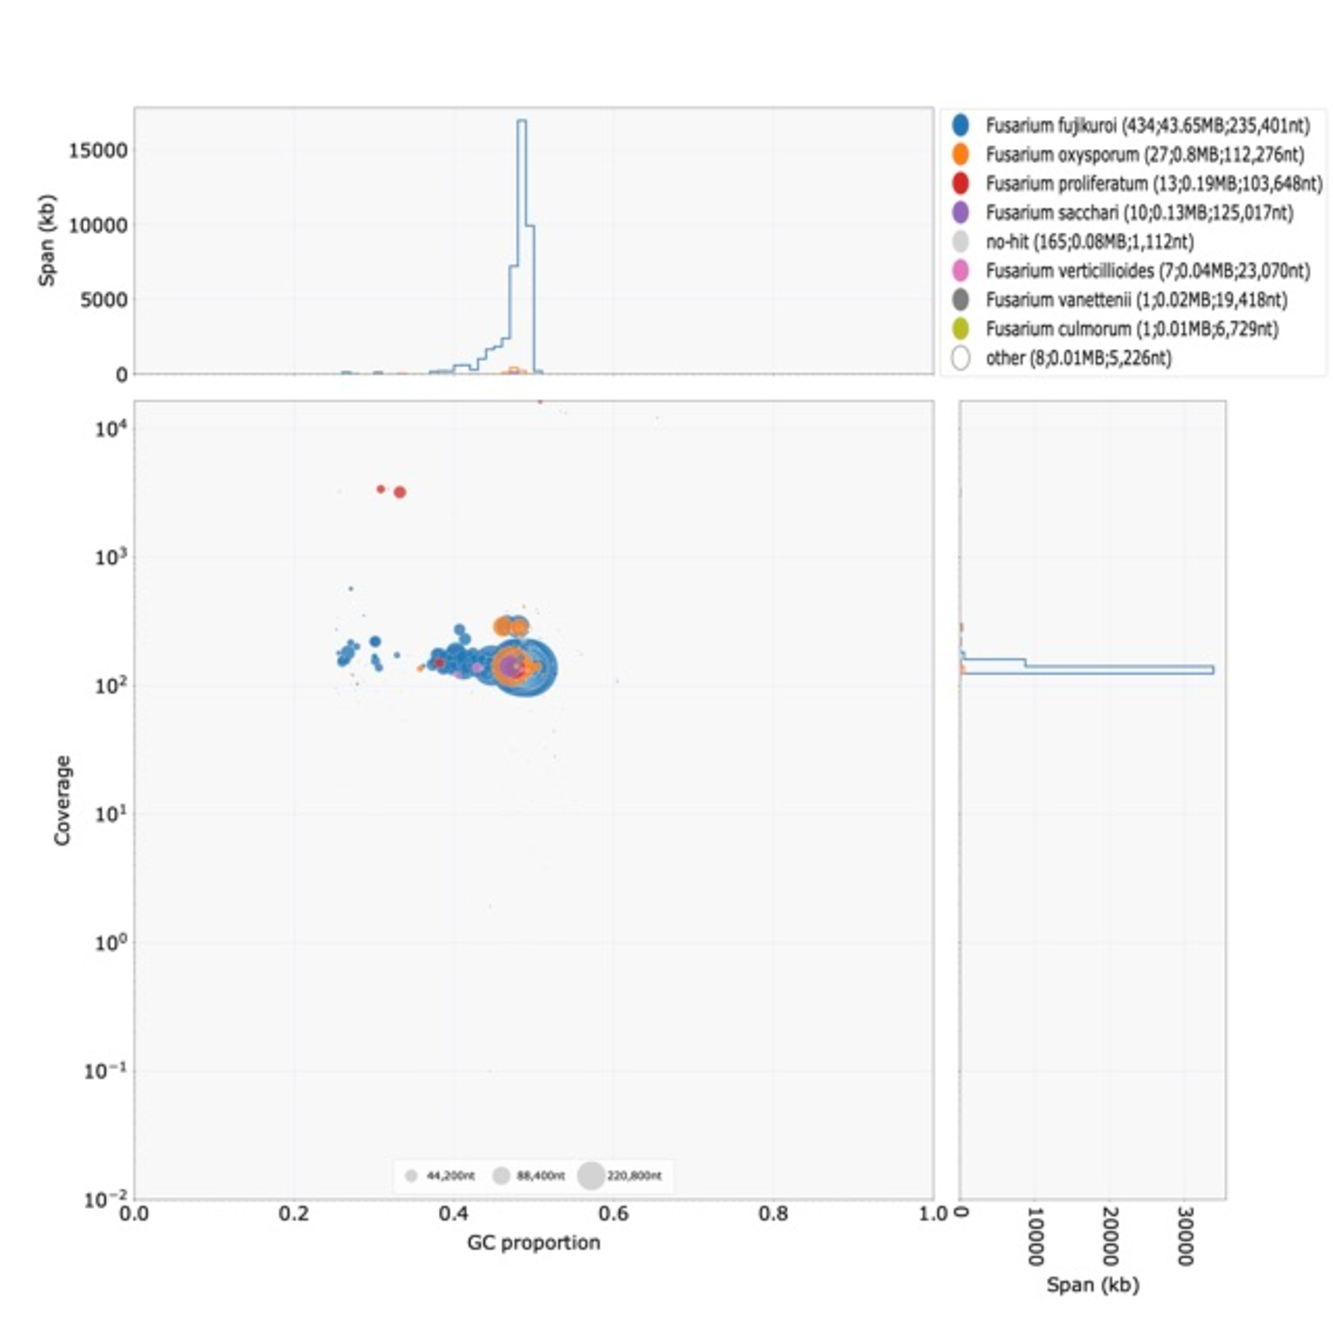
\includegraphics[width=\textwidth]{Figures/TNAU_S16.species.blobplot.pdf}
        \caption{}
        \label{fig:BlobPlot-S16}
    \end{subfigure}
    \begin{subfigure}[]{0.9\textwidth}
        \centering
        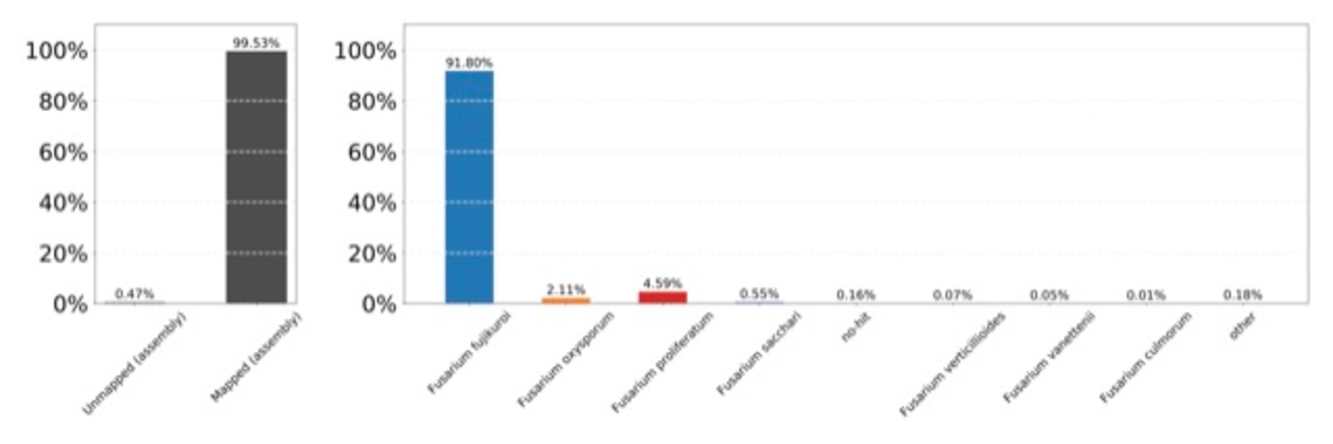
\includegraphics[width=\textwidth]{Figures/TNAU_S16.blobtools.blobDB.json.bestsum.species.p8.span.100.blobplot.read_cov.bam0.pdf}
        \caption{}
        \label{fig:BlobPlot_readcov-S16}
    \end{subfigure}
    \caption[BlobTools visualisations of the S16 assembly]{\textbf{BlobTools visualisations of the S16 assembly shows \acf{Ff} is the most common species hit.}
        \subref{fig:BlobPlot-S16} BlobPlot of S16. Sequences in the assembly are depicted as circles, with diameter proportional to sequence length and coloured by taxonomic annotation based on BLASTN (v2.9.0+) of NCBI nt database.
        \subref{fig:BlobPlot_readcov-S16} Read coverage plot of the S16 assembly. Mapped reads are shown by taxonomic group at the rank of species.}
        \label{fig:S16:BlobTools}
\end{figure}
%%%%%%%%%%%%%%%%%%%%%%%%%%
%%%%% S32 BlobTools %%%%%%
%%%%%%%%%%%%%%%%%%%%%%%%%%
\begin{figure}[hp!]
    \centering
    \begin{subfigure}[]{0.9\textwidth}
        \centering
        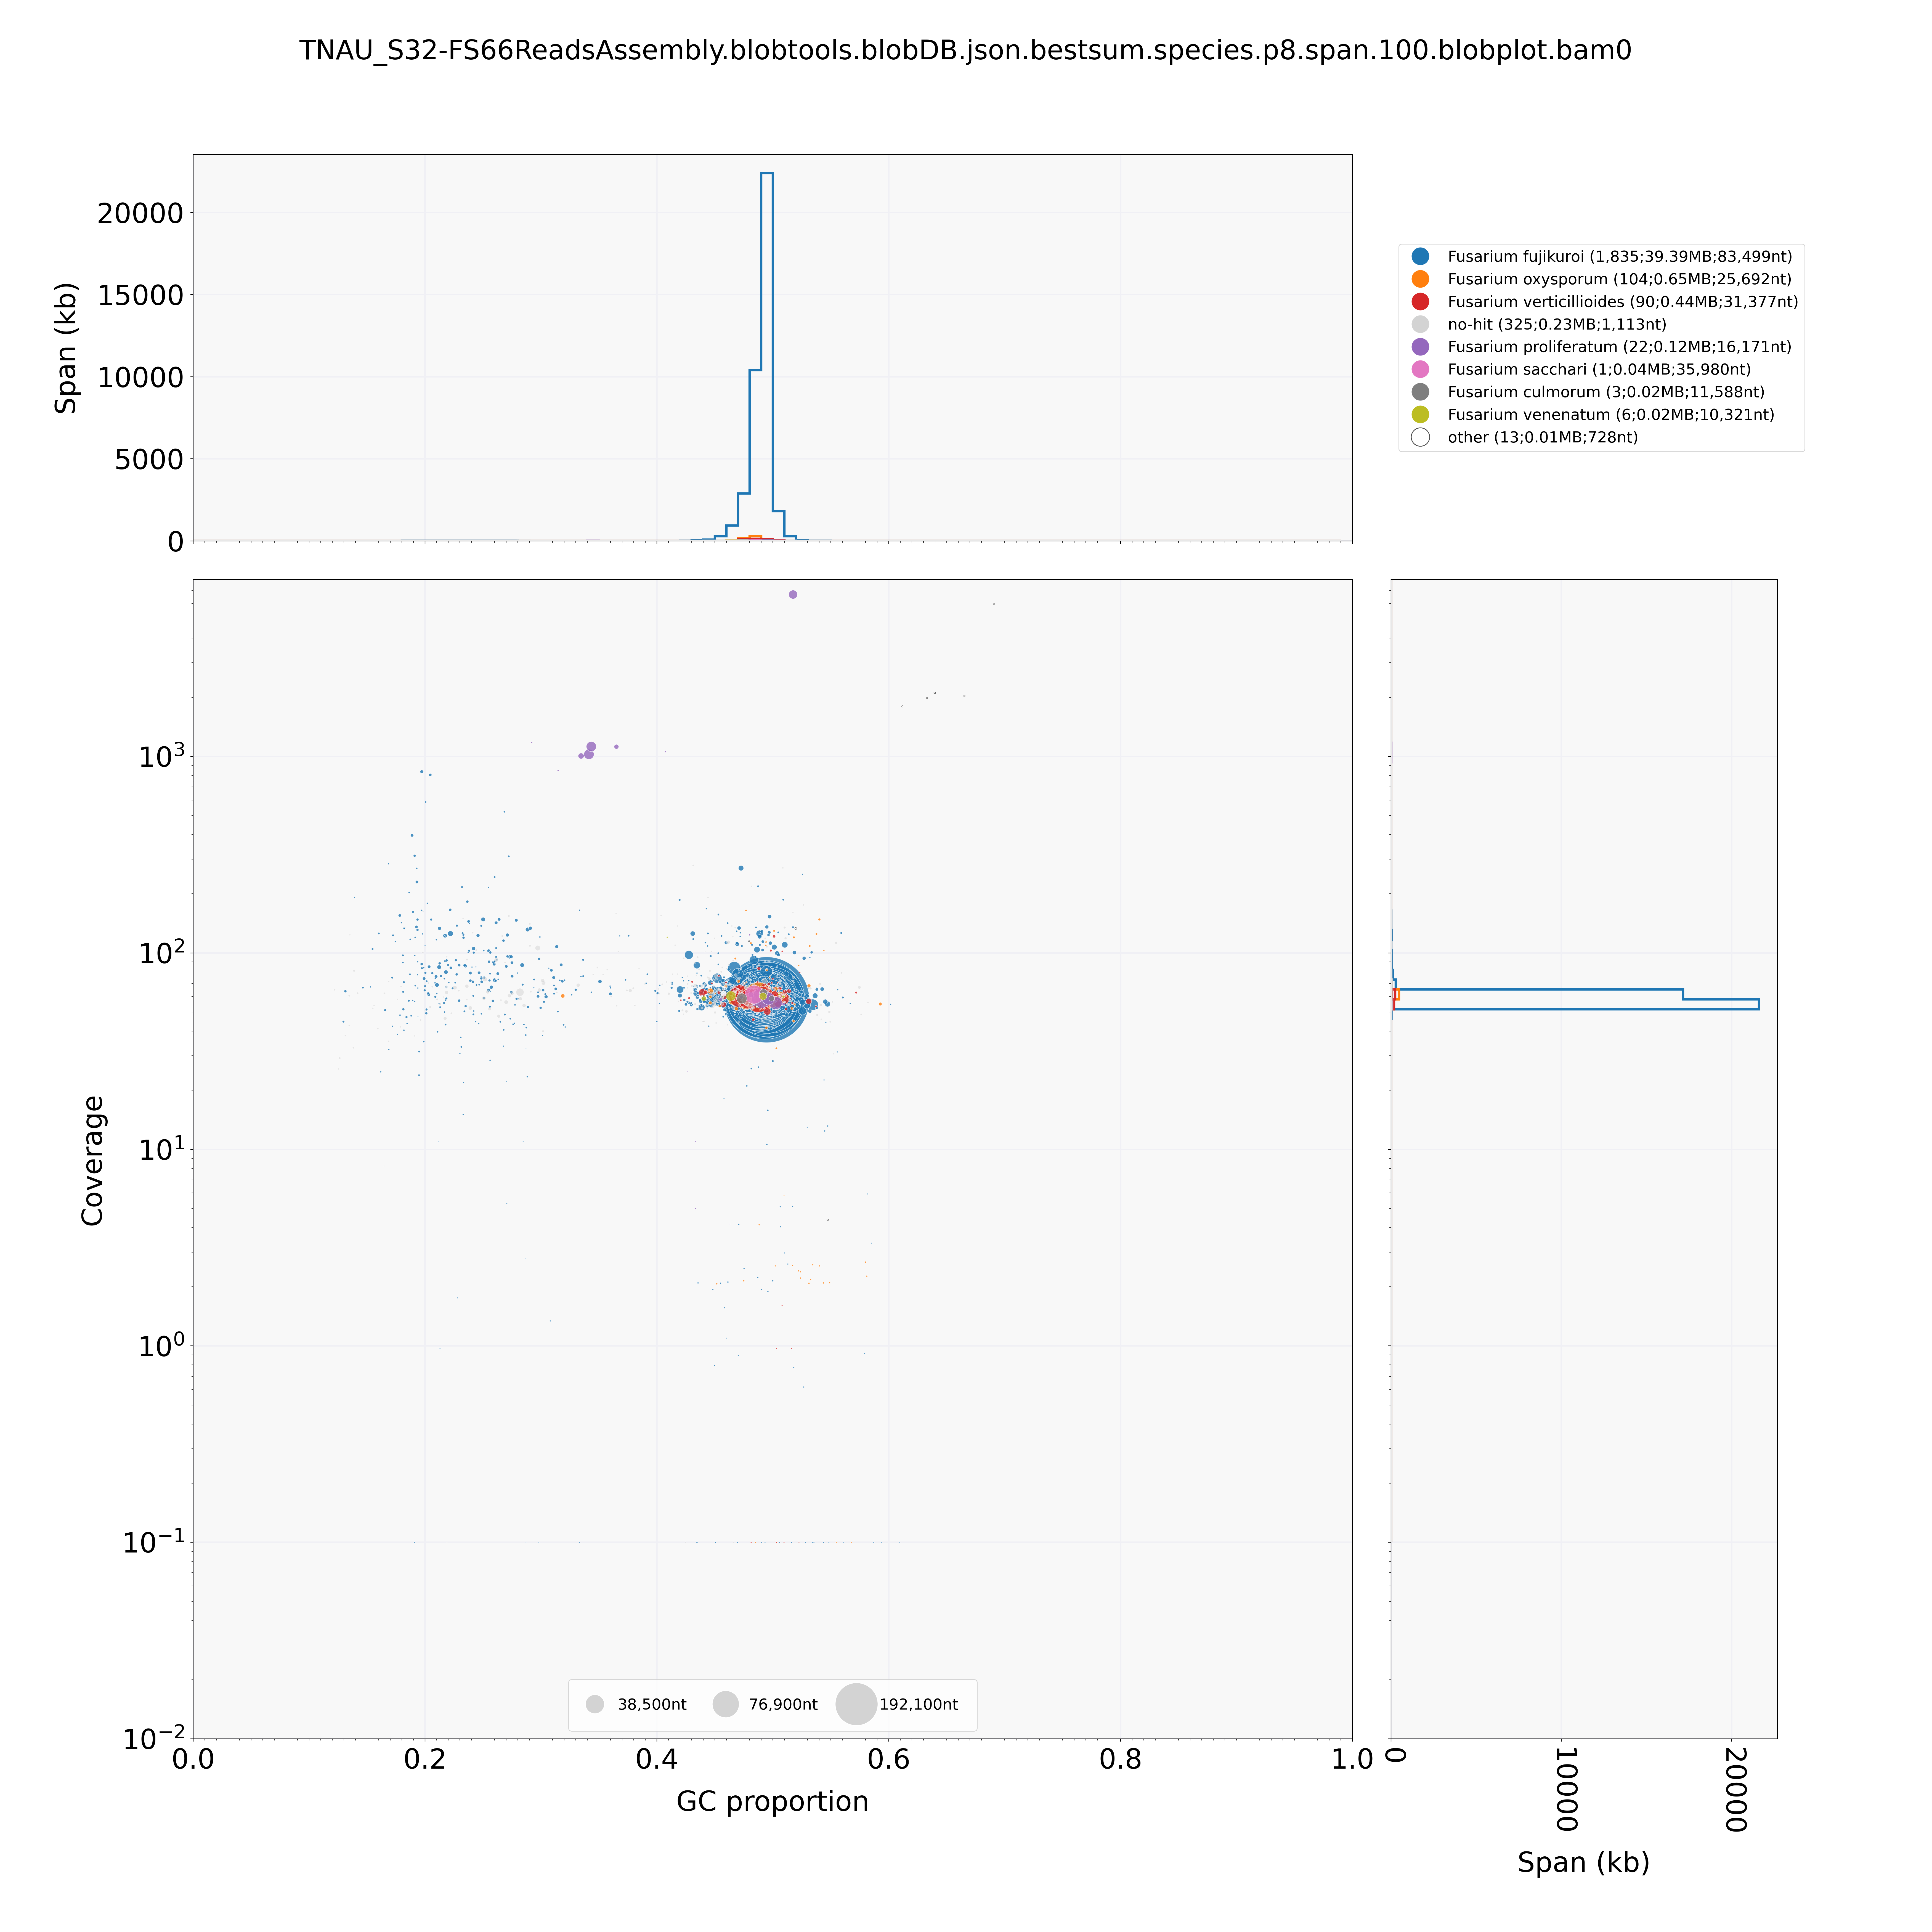
\includegraphics[width=\textwidth]{Appendices/TNAU_S32-FS66ReadsAssembly.blobtools.blobDB.json.bestsum.species.p8.span.100.blobplot.bam0.png}
        \caption{}
        \label{fig:BlobPlot-S32}
    \end{subfigure}
    \begin{subfigure}[]{0.9\textwidth}
        \centering
        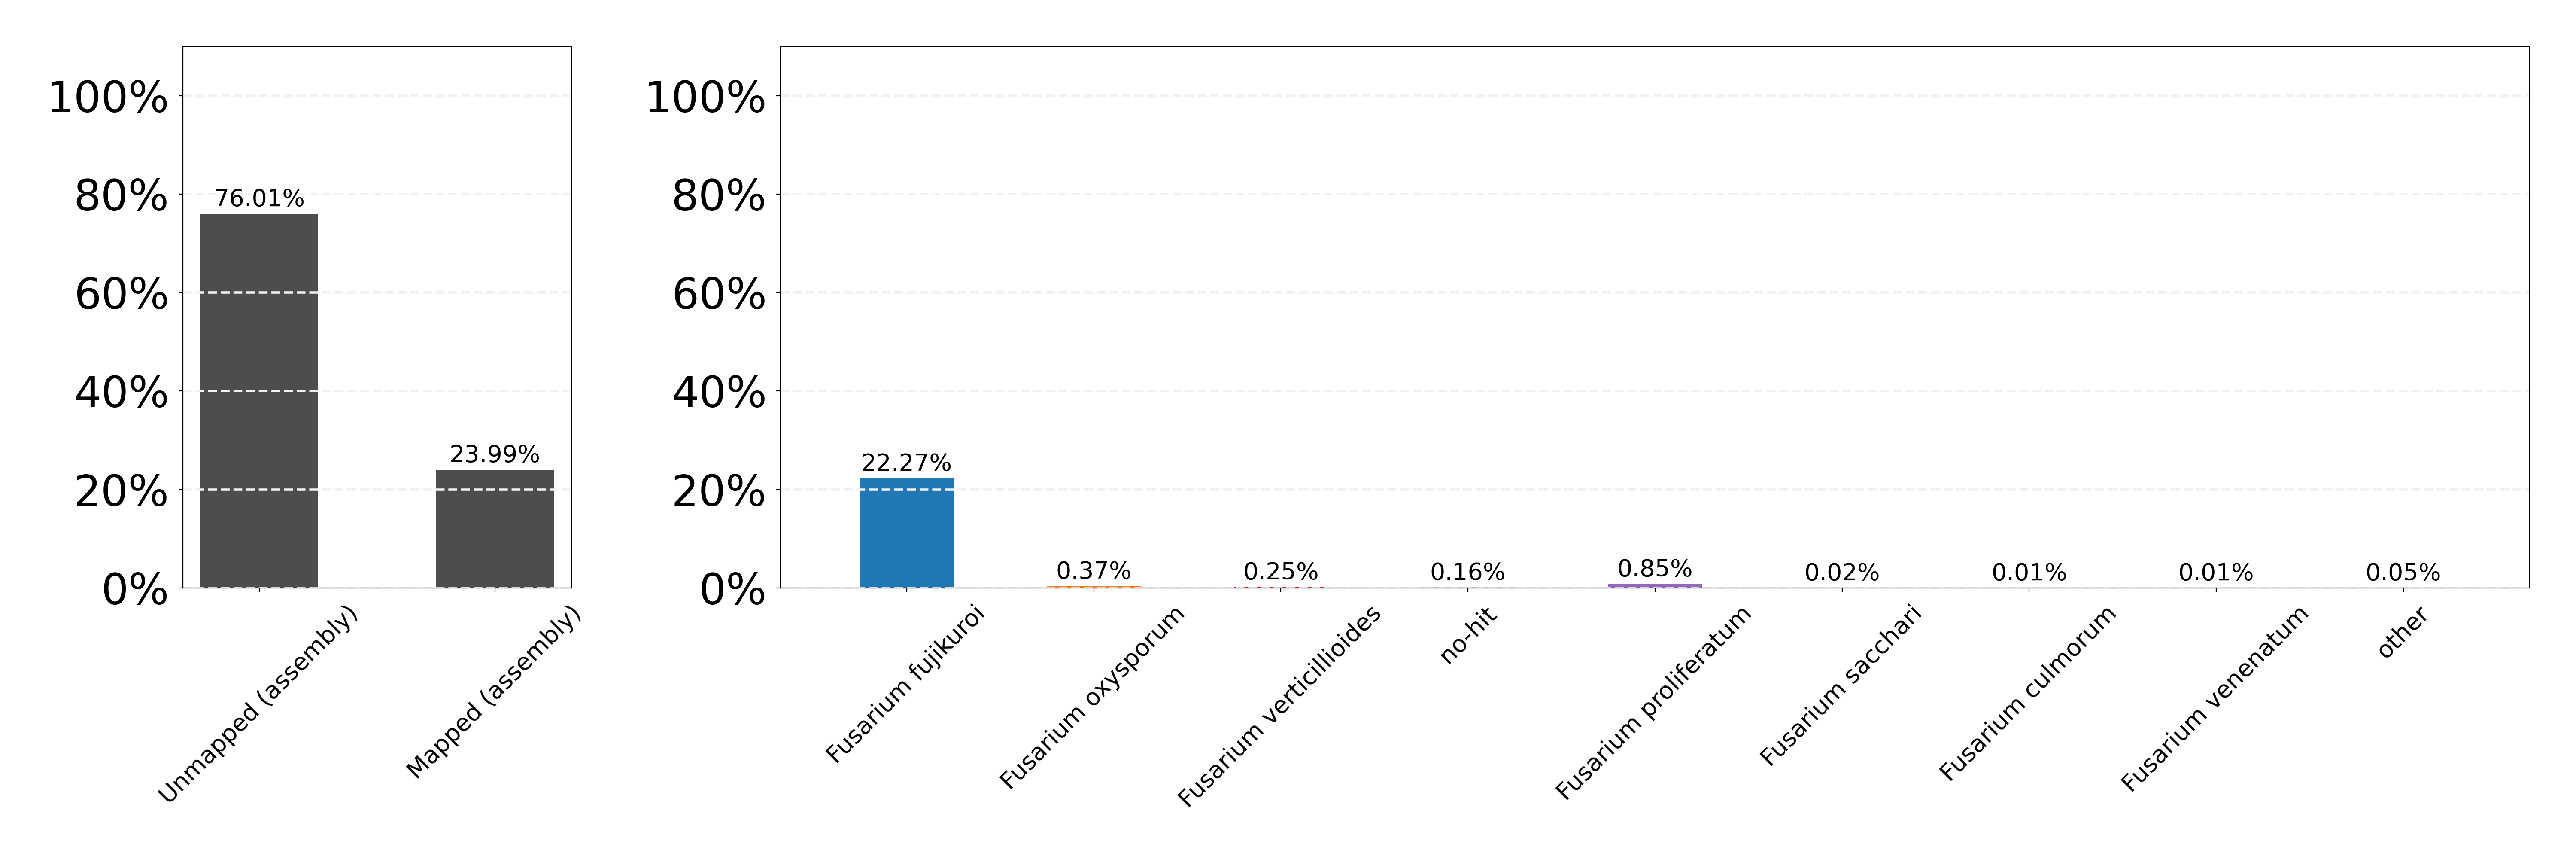
\includegraphics[width=\textwidth]{Appendices/TNAU_S32-FS66ReadsAssembly.blobtools.blobDB.json.bestsum.species.p8.span.100.blobplot.read_cov.bam0.png}
        \caption{}
        \label{fig:BlobPlot_readcov-S32}
    \end{subfigure}
    \caption[BlobTools visualisations of the S32 assembly]{\textbf{BlobTools visualisations of the S32 assembly shows \acf{Ff} is the most common species hit.}
        \subref{fig:BlobPlot-S32} BlobPlot of S32. Sequences in the assembly are depicted as circles, with diameter proportional to sequence length and coloured by taxonomic annotation based on BLASTN (v2.9.0+) of NCBI nt database.
        \subref{fig:BlobPlot_readcov-S32} Read coverage plot of the S16 assembly. Mapped reads are shown by taxonomic group at the rank of species.}
        \label{fig:S32:BlobTools}
\end{figure}
%%%%%%%%%%%%%%%%%%%%%%%%%%
%%%%%% S6 BlobTools %%%%%%
%%%%%%%%%%%%%%%%%%%%%%%%%%
\begin{figure}[hp!]
    \centering
    \begin{subfigure}[]{0.9\textwidth}
        \centering
        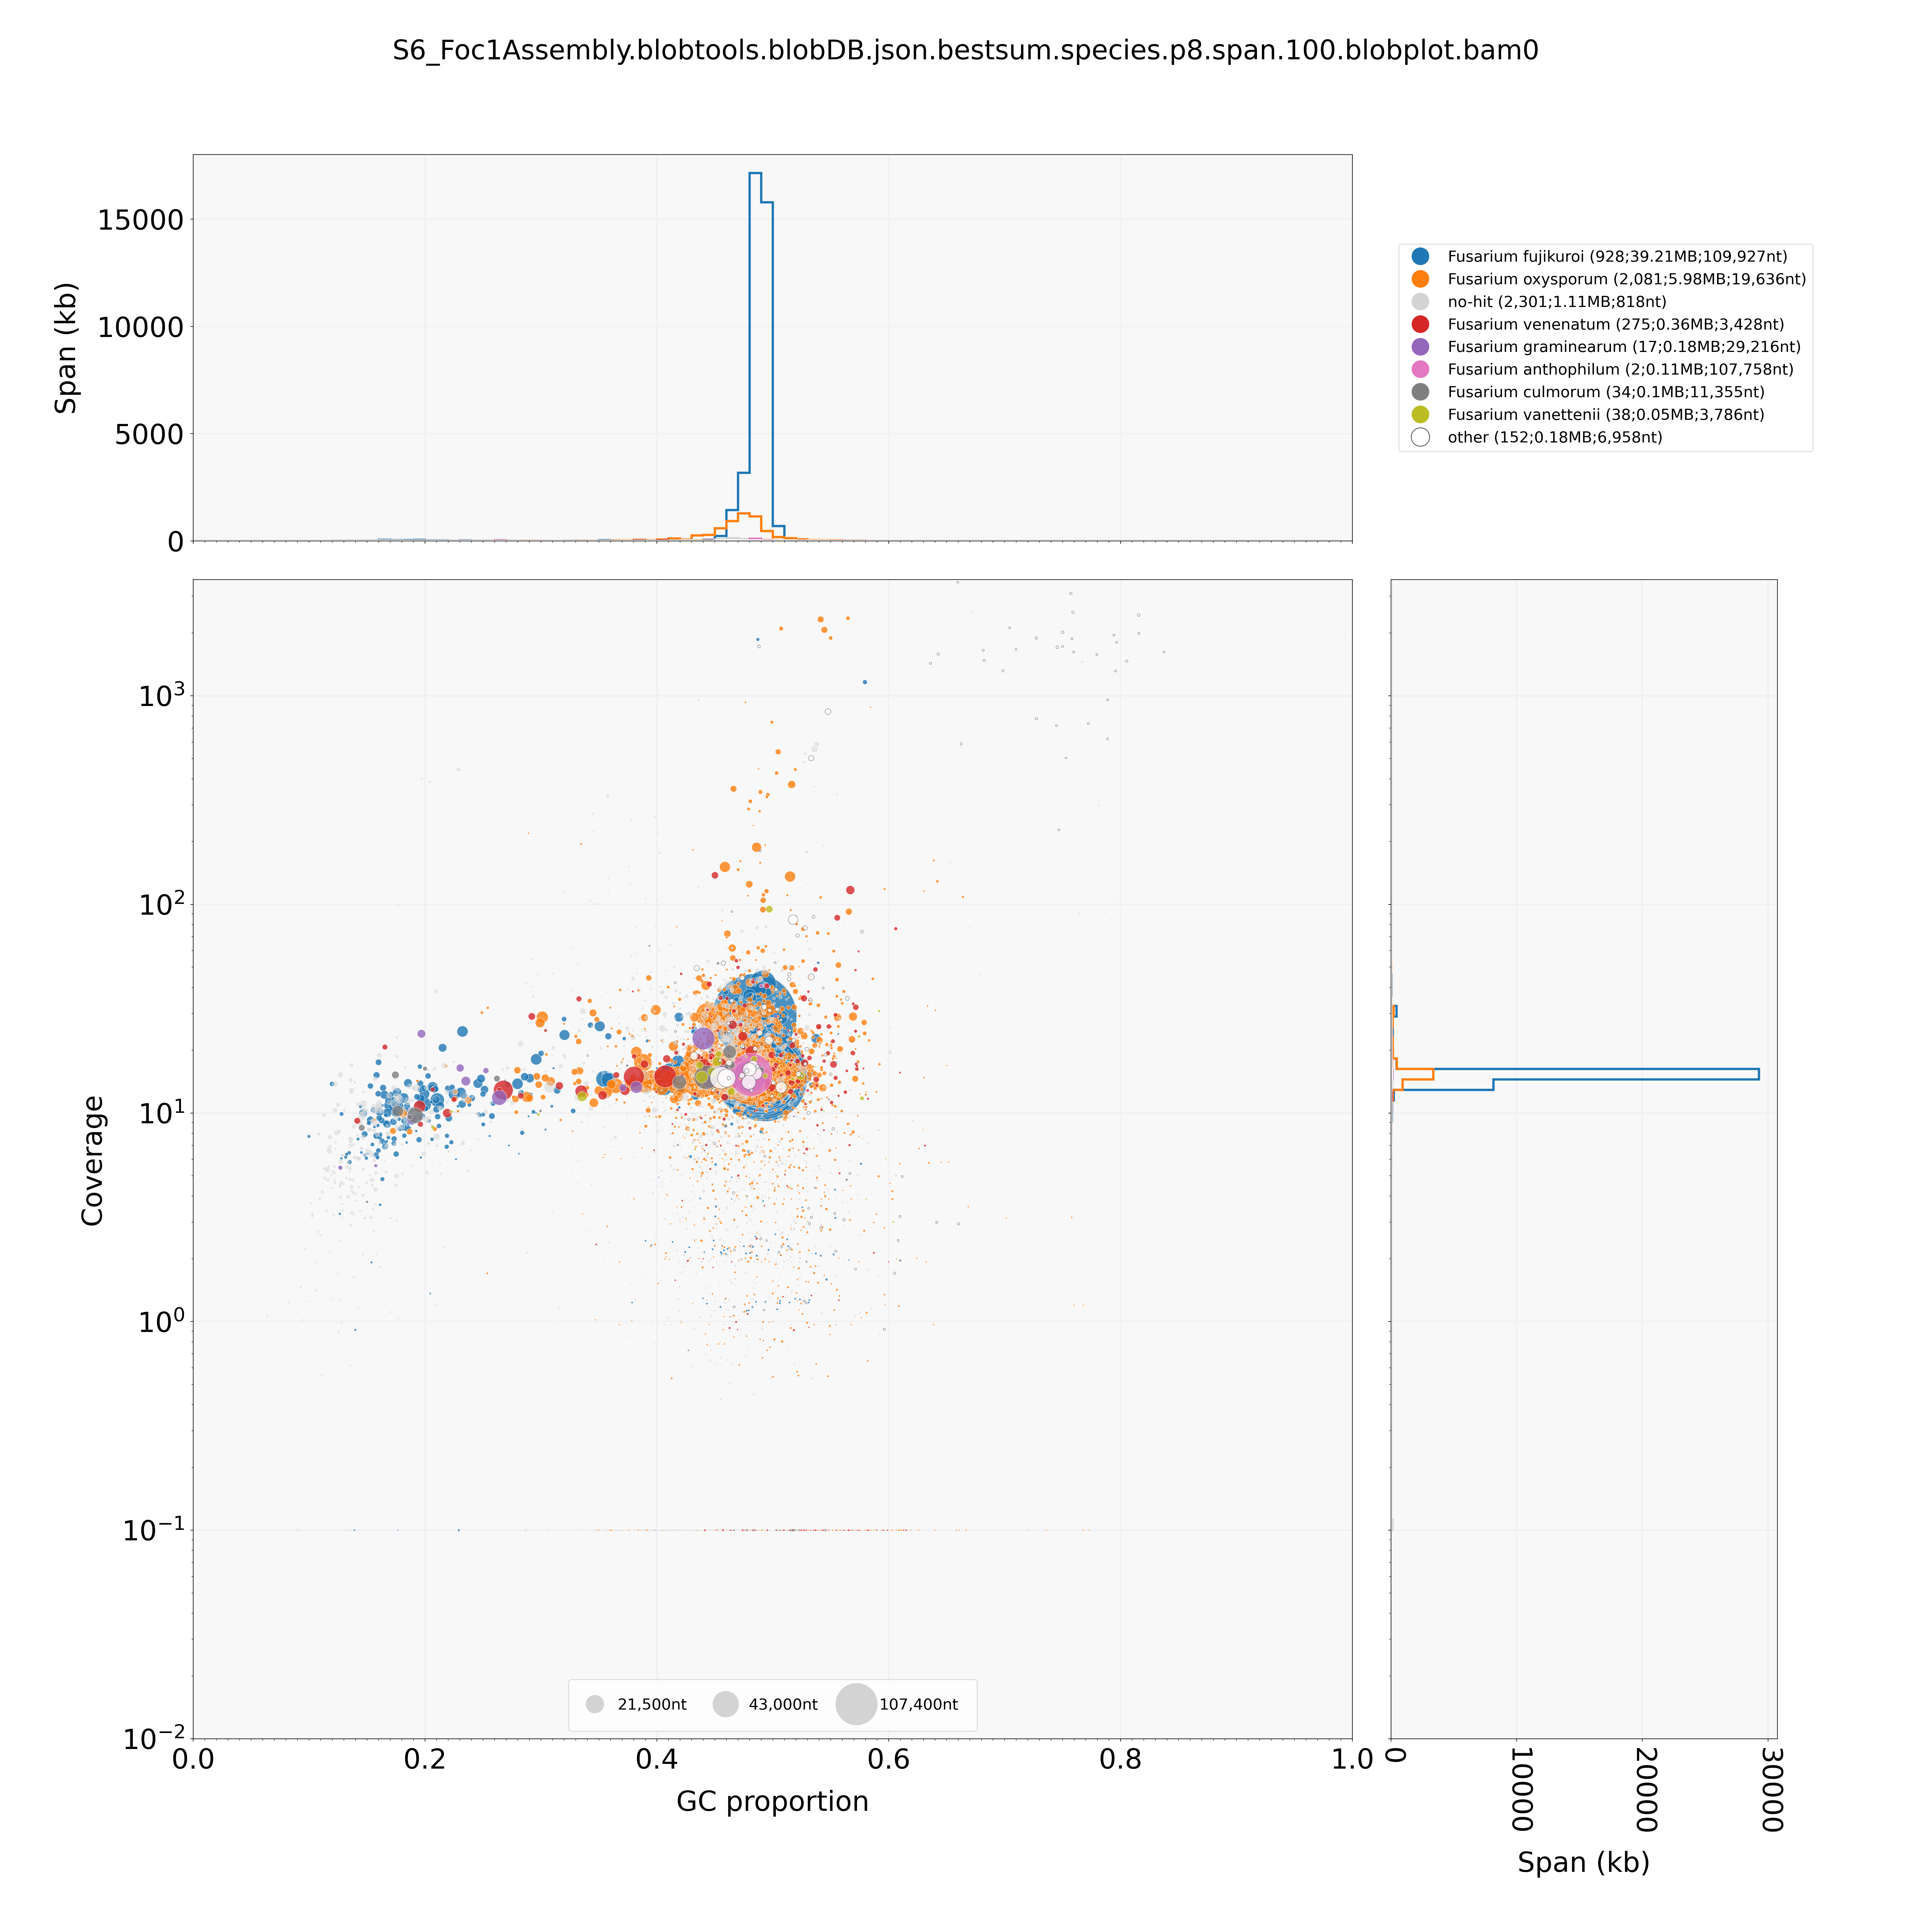
\includegraphics[width=\textwidth]{Appendices/S6_Foc1Assembly.blobtools.blobDB.json.bestsum.species.p8.span.100.blobplot.bam0.png}
        \caption{}
        \label{fig:BlobPlot-S6}
    \end{subfigure}
    \begin{subfigure}[]{0.9\textwidth}
        \centering
        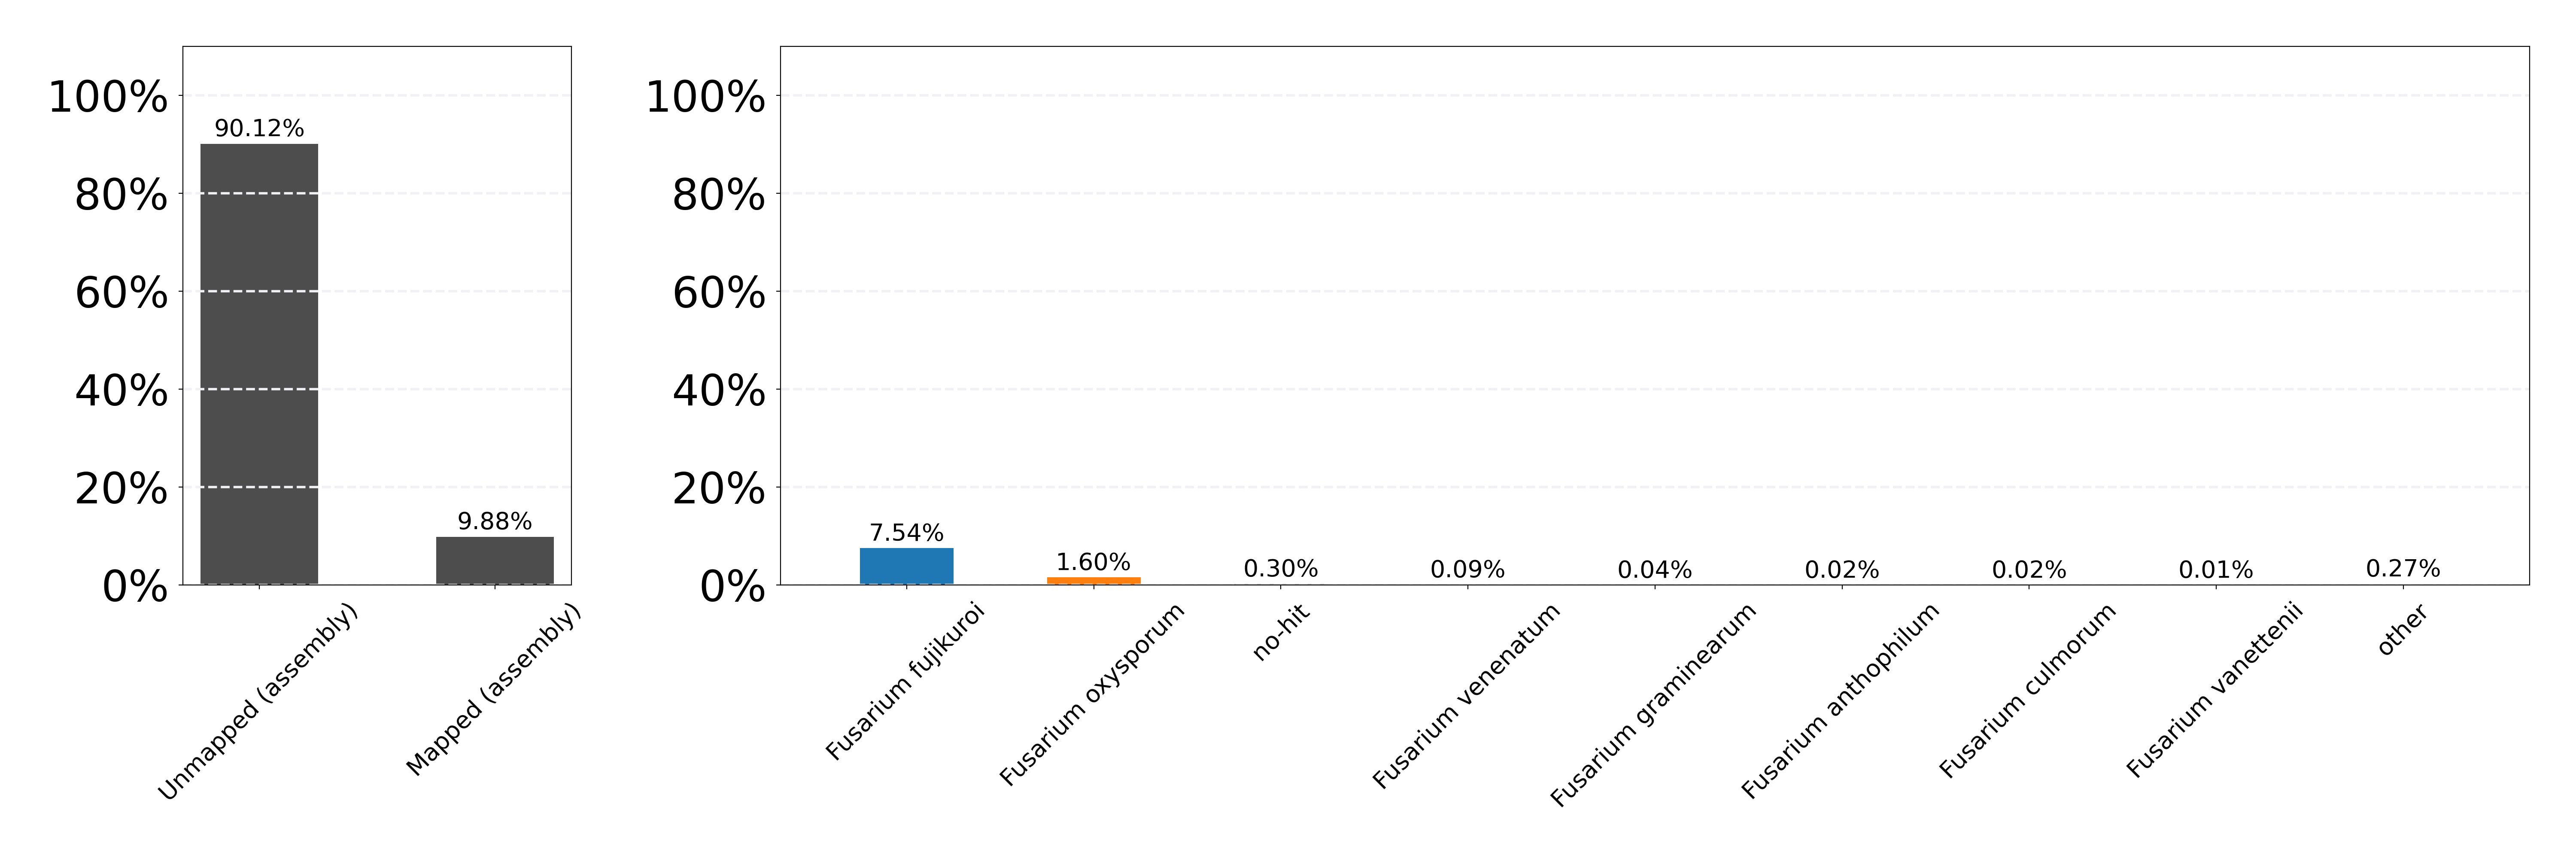
\includegraphics[width=\textwidth]{Appendices/S6_Foc1Assembly.blobtools.blobDB.json.bestsum.species.p8.span.100.blobplot.read_cov.bam0.png}
        \caption{}
        \label{fig:BlobPlot_readcov-S6}
    \end{subfigure}
    \caption[BlobTools visualisations of the S6 assembly]{\textbf{BlobTools visualisations of the S6 assembly.}
        \subref{fig:BlobPlot-S6} BlobPlot of S6. Sequences in the assembly are depicted as circles, with diameter proportional to sequence length and coloured by taxonomic annotation based on BLASTN (v2.9.0+) of NCBI nt database.
        \subref{fig:BlobPlot_readcov-S6} Read coverage plot of the S6 assembly. Mapped reads are shown by taxonomic group at the rank of species.}
        \label{fig:S6:BlobTools}
\end{figure}



Following BlobTools (v1.1.1) analysis, contaminated contigs (assigned to species other than \textit{Fusarium}) were removed. The  S6, S16, S32, and SY-2 contaminant-filtered genome assemblies contained 6,048, 768, 2,443, and 408 contigs, respectively. Coverage varied from 16x for S6 genome assembly to 148x for S16 genome assembly (Table~\ref{tab:TNAUAssemblyStats}), and percentage GC content ranged from 47.53\% (S16) to 48.85\% (S32). All genome assemblies were between 40Mb and 50Mb in length and contained 15,719 to 17,891 predicted protein coding genes. Genome completeness was assessed using \ac{busco} (v5.4.6) with the hypocreales\_odb10 dataset. SY-2, S6, S16, and S32 genome assemblies contained 99.60\%, 97.50\%, 97.40\%, and 97.40\% intact, single-copy orthologs, respectively. 

% Please add the following required packages to your document preamble:
% \usepackage{multirow}
% \usepackage{longtable}
% Note: It may be necessary to compile the document several times to get a multi-page table to line up properly
\begingroup
\setlength{\tabcolsep}{20pt} % Default value: 6pt
\renewcommand{\arraystretch}{0.9}
\setlength\LTcapwidth{\textwidth} % default: 4in (rather less than \textwidth...)
\setlength\LTleft{0pt}            % default: \parindent
\setlength\LTright{0pt}           % default: \fill
\begin{longtable}[c]{ccccc}
\caption[Summary statistics of TNAU genome assemblies.]{\textbf{Summary statistics of TNAU genome assemblies. }\textit{De novo} assemblies generated using SPAdes (version 3.14.1) with all raw reads supplied by Tamil Nadu Agricultural University. }
\label{tab:TNAUAssemblyStats}\\
\hline
\multirow{\textbf{\begin{tabular}[c]{@{}l@{}}Assembly\\Statistic\end{tabular}}} & \multicolumn{4}{c}{\textbf{TNAU Isolate Assembly}} \\ \cline{2-5} 
                    & \textbf{SY-2}    & \textbf{S6} & \textbf{S16} & \textbf{S32} \\ \hline
\endfirsthead
%
\multicolumn{5}{c}%
{{\bfseries Table \thetable\ continued from previous page}} \\
\endhead
%
Number of contigs   & 441      &                & 768       & 2443        \\
Largest contig (Mb) & 0.87     &                & 0.88      & 0.77        \\
Total length (Mb)   & 44.35    &                & 44.86     & 40.92       \\
GC (\%)             & 47.97    &                & 47.53     & 48.85       \\
N50 (bp)            & 221769   &                & 234991    & 78523       \\
L50                 & 57       &                & 60        & 109         \\
Mapped Reads (\%)   & 99.6     &                & 99.53     &             \\
Mean Coverage       & 73x      &                & 148x      &             \\ 
BUSCO (\%)          & 99.6     &                & 97.4      & 97.4        \\\hline  


\end{longtable}
\endgroup

\subsubsection{Contamination in the S6 and S32 raw read data}
\label{sec:BlobToolsOfS6S32-allreads}

Since a high proportion of the genomic reads  from isolates S6 and S32 originating from the to bacterium \textit{S. maltophilia}, I performed \textit{de novo} assembly, specifically for evaluating taxonomic partitioning with BlobTools (v1.1.1). These genome assemblies generated from both unfiltered and unmapped genomic raw reads contained 100,147 and 1,048 contigs, recorded  97.70\% and 97.70\% \ac{busco} intact single-copy orthologs, were 97.64Mb and 49.62Mb in length and had a GC content of 46.75\% and 49.80\% for S6 and S32, respectively. The S6 genome assembly generated using all raw reads was much larger than is typical for a \ac{Fo} assembly and was highly fragmented. Both genome assemblies contained a large number of contigs that had either no hits or were assigned to genera other than \textit{Fusarium}.  For instance, 93,702 contigs from the S6 genome assembly had no hits and over 2,000 contigs were assigned to species other than \textit{Fusarium}, though 814 and 647 of the contigs were assigned to \ac{Ff} and \ac{Fo}, respectively (Appendix \ref{fig:S6:BlobToolsAllreads}). The majority of contigs from the S32 \textit{de novo} genome assembly had the greatest sequence similarity to \textit{Fusarium} species, particularly \ac{Ff} (n=241), although 350 contigs had no-hits and 200 contigs were assigned to \textit{Stenotrophomonas} species, as was observed in the \acs{blast}N search of unmapped raw reads (Appendix \ref{fig:S32:BlobToolsAllreads}). 

\subsection{\acl{tef} and \acl{rbp2} reveal novel clade of \textit{Fusarium}}

 Sequences encoding the common \textit{Fusarium} barcodes, \ac{tef}  and \acf{rbp2}, were extracted from the \ac{tnau} isolates and used to infer a maximum-likelihood phylogeny (Figure: \ref{fig:TEF1aPhylo}). S6 falls within one of the \ac{Focub1} clades in the \acs{tef} and \ac{rbp2} phylogeny (Appendix \ref{fig:rbp2Phylo}). \Ac{tef} and \ac{rbp2} sequences from the S16 genome assembly sit within the same clade as the SY-2 and reference \ac{Fs} \ac{tef} and \ac{rbp2} sequences which, taken together with the raw read mapping data, suggests these isolates may be strains of \ac{Fs} pathogenic towards banana. Based on the \ac{tef} and \ac{rbp2} phylogenies, S32 appears to be a sister lineage of \ac{Fs}. S32 groups with the novel species, \textit{F. mindanaoense}, recently proposed by  \textcite{Nozawa2023} infecting Cavendish banana in the Philippines. 

These extracted \ac{tef} sequences were also searched against the Fusariod-ID MSLT and \ac{ncbi} BLAST databases for similar sequences. A search of the \ac{ncbi} database revealed that the \ac{tef} sequence extracted from the S16 genome assembly best scoring hits were for \ac{Fs} (Table \ref{tab:Tef1-NCBIdb}). Further, the Fusariod MSLT database best scoring hits for the \ac{tef} sequence extracted from the S16 genome assembly were for sequences from the \ac{FFSC}, in which \ac{Fs} can be found (Appendix \ref{tab:Tef1-MLSTdb}). Searches for the S6 isolate extracted \ac{tef} sequence suggest S6 belongs to the \ac{FOSC}. Although there were matches for \ac{Focub} \ac{tef} sequences, these were not in the top 3 results from searches of both databases for the S6 \ac{tef} sequence. No matches were found for the S32 extracted \ac{tef} sequences in the Fusarioid-ID MSLT database, and hits against the \ac{ncbi} GenBank database were for \ac{tef} sequences from \ac{Ff}. 

% Please add the following required packages to your document preamble:
% \usepackage{multirow}
% \usepackage{graphicx}
% \usepackage{lscape}
\begin{table}[h!]
\centering
\captionsetup{width=\linewidth} 
\caption[\Ac{tnau}\acf{tef} \acf{ncbi} and Fusariod-ID MSLT database searches.]{\textbf{Best hits of extracted \acf{tef} sequences from the \acf{tnau} isolate \textit{de novo} assemblies using \ac{ncbi} web-BLASTN.}}
\label{tab:Tef1-NCBIdb}
\resizebox{\columnwidth}{!}{%
\begin{tabular}{cccc}
\multicolumn{1}{l}{\multirow{2}{*}{\textbf{TNAU Isolate Assembly}}} & \multicolumn{3}{c}{\textbf{NCBI database}}                                        \\ \cline{2-4} 
\multicolumn{1}{l}{}                                       & Hit 1                    & Hit 2                    & Hit 3                       \\ \hline
\textbf{S6}                            & \textit{F. o.} isolate 170 & \textit{F. o.} f. sp. \textit{koae} & \textit{F. o.} f. sp. \textit{dianthi} \\
\textbf{S16}                                               & \textit{F. sacchari} CBS:147.25   & \textit{F. sacchari} NRLL 66326  & \textit{F. globosum} CBS:428.97      \\
\textbf{S32}                             & \textit{F. fujikuroi} I1.3        & \textit{F. fujikuroi} IMI 58289   & \textit{F. fujikuroi} Augusto2 \\ 
\textbf{SY-2} & \textit{F. fujikuroi} I1.3        & \textit{F. fujikuroi} IMI 58289   & \textit{F. fujikuroi} Augusto2 \\ \hline     
\end{tabular}%
}
\end{table}

\begin{figure}[htp!]
    \centering
    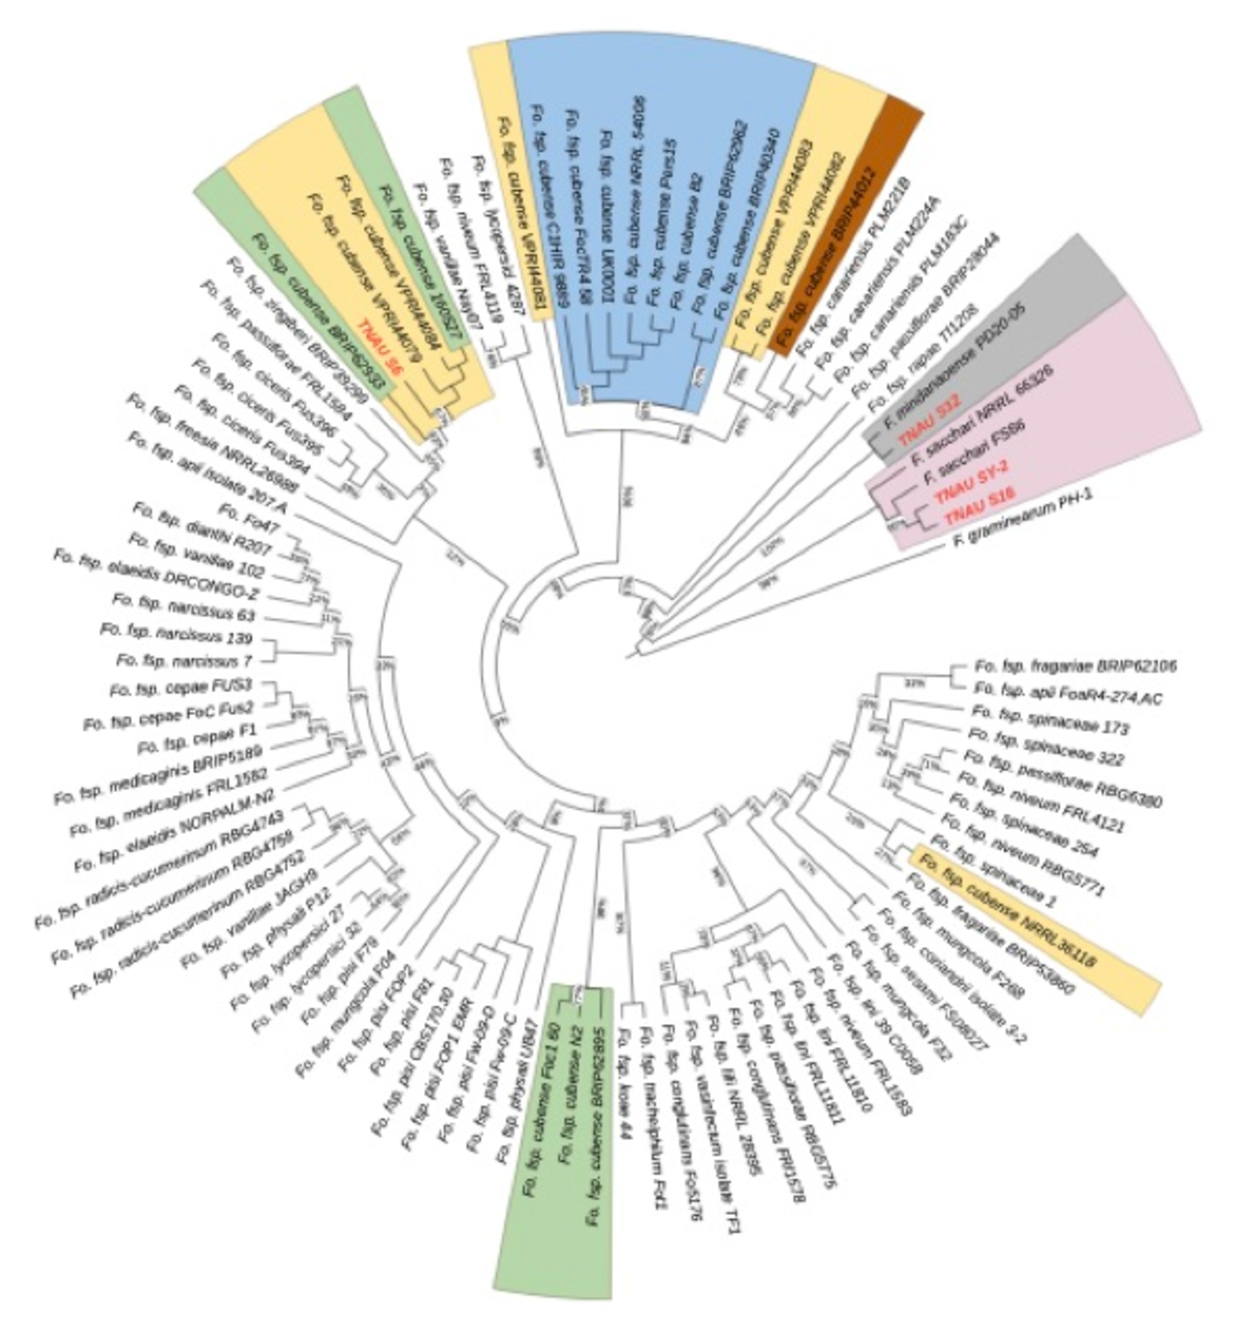
\includegraphics[width=14cm]{Figures/TEF1-aPhylo3.pdf}
    \caption[\Acl{tef} phylogeny of \acl{tnau} \textit{Fusarium} isolates.]{\textbf{\Acl{tef} phylogeny of \acl{tnau} \textit{Fusarium} isolates.} \Ac{tnau} isolates S16, S32 and SY-2 sit within the \acf{FFSC} clade. The \ac{tef} sequences from \ac{tnau} are shown in red text. The \acf{Fs} clade is shown in pink. \Acf{Focub4} \ac{tef} sequences are in blue and \acf{str4} in brown. \Acf{Focub1} \ac{tef} sequences are shown in green. The \ac{tef} sequences from \acf{Focub} genome assemblies with race not recorded are shown in yellow. Percentages represent values from 1000 bootstrap replicates. The tree is rooted through \textit{Fusarium graminearum} PH-1 \ac{tef}.}
    \label{fig:TEF1aPhylo}
\end{figure}
\bigskip

\subsection{Identification of pathogen-specific features}

\subsubsection{\textit{Secreted In Xylem} gene distribution suggest \ac{tnau} isolates S16, S32, and SY-2 are not \ac{Focub} }

\Acp{sixg} are the only family of effectors currently confirmed in \ac{Fo} \parencite{Armitage2018, Czislowski2018}. \Ac{sixg} homologues (\textit{SIX1-SIX14}) were identified in the \ac{tnau} genome assemblies, alongside publicly available genome assemblies of \ac{Focub} (n=14), \ac{Fs} (n=2), \ac{Fo} \acp{fsp} (n=7), a \ac{Fo} endophyte, and a \textit{F. graminearum} genome assembly. No \acp{sixg} were identified in the S32 genome assembly. A \textit{SIX2} homologue was identified in S16,  SY-2  and  \ac{Fs} genome assemblies (Figure \ref{fig:SixTNAU}), and no other \acp{sixg} were identified. The S6 genome assembly clustered with other \ac{Focub1} isolates that have \textit{SIX1, SIX4, SIX6}, and \textit{SIX9} homologues identified, although, \textit{SIX13} is not present in this genome assembly. Interestingly, no \acp{sixg} were identified in the \ac{Focub1} genome genome assembly, Foc1 60, which clustered with S32, as well as the \ac{Fo} endophyte and \textit{F. graminearum} genome assemblies. 

As homologues of \textit{SIX1, SIX2, SIX4, SIX6}, and \textit{SIX9} were identified in the \ac{tnau} genome assemblies, these sequences were extracted for phylogenetic analysis.  One copy of \textit{SIX9} was identified in the S6 genome assembly, which was shared with all \ac{Focub} genome assemblies (Figure \ref{fig:FusSIX9}). A further copy of \textit{SIX9} was found in each of the \ac{Focub4} genome assemblies and assemblies for VPRI44081, VPRI44082, VPRI44083 (race not known). In the \textit{SIX1} phylogeny, the S6 \textit{SIX1}  falls within the same clades as the \textit{SIX1} from \ac{Focub1} N2 and 160527 genome assemblies, and the \ac{Focub1} assemblies which have no race data available: VPRI44079, VPRI44082, VPRI44083, VPRI44084 (Figure \ref{fig:FusSIX1}), but the number of copies of \textit{SIX1} identified varies between isolate genome assembly. The same can also be observed for \textit{SIX4} and \textit{SIX6} (\ref{fig:FusSIXMultiPhylo}). \textit{SIX2} was not identified in the S6 assembly or the \ac{Focub1} assemblies. However, it was identified in the S16 and SY-2, \ac{Fs} and other \ac{Focub} genome assemblies. The SY-2 and S16 \textit{SIX2} sequences fall within the \ac{Fs} clade in the \textit{SIX2} phylogeny (Figure \ref{fig:FusSIX2}).

\begin{figure}[htp!]
  \centering
  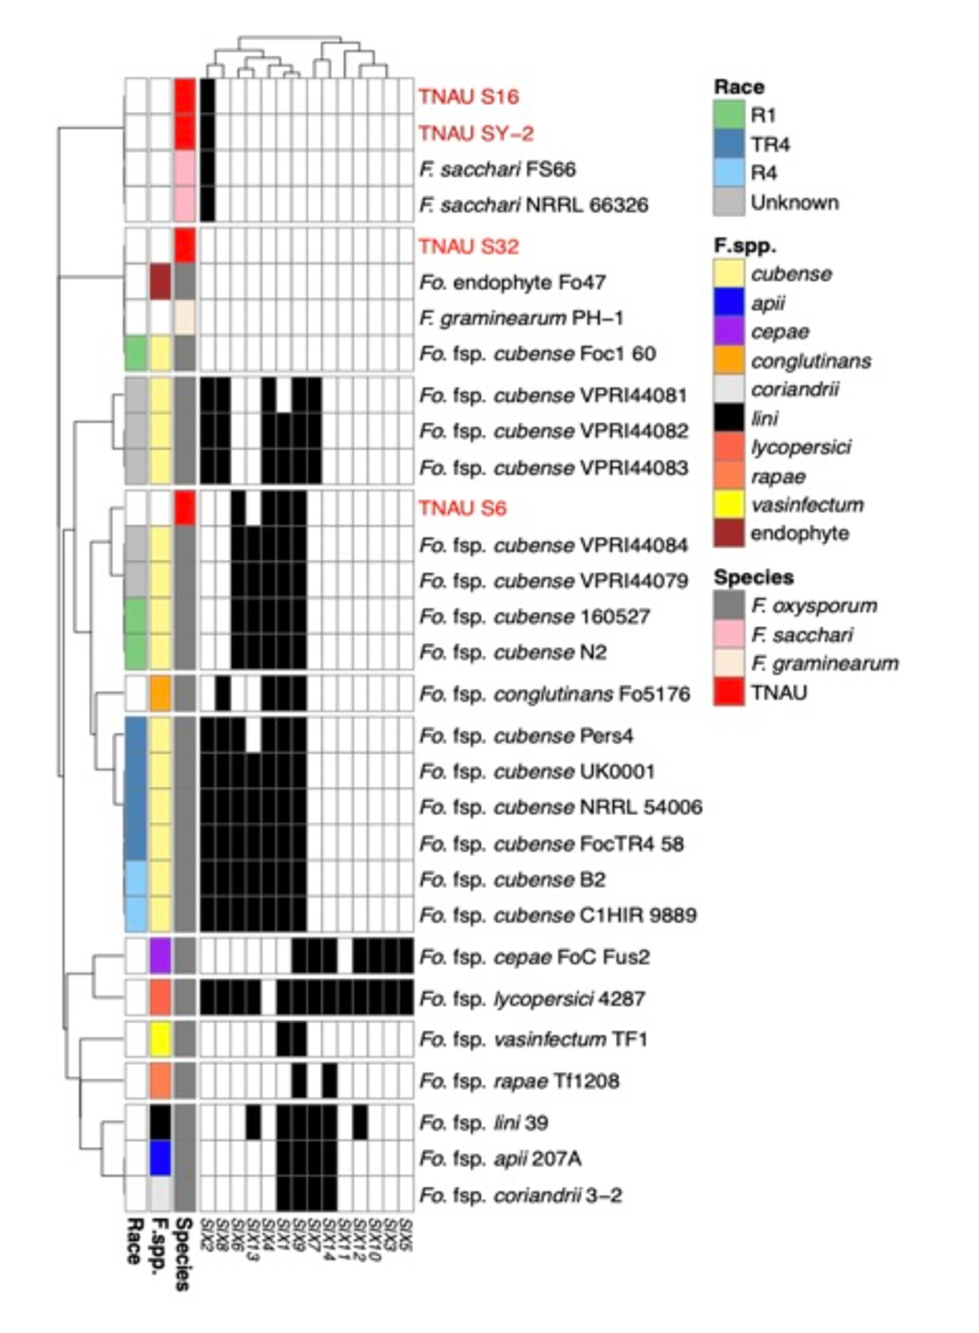
\includegraphics[width=15cm]{Figures/SIX_Heatmap.pdf}
  \caption[Binary distribution of \textit{SIX} genes across Fusarium tnau genome assemblies]{\textbf{Binary distribution of \textit{SIX} genes across Fusarium tnau genome assemblies}. \aclp{sixg} identified using TBLASTN (cut off 1\-e\textsuperscript{6}) using SIX genes from \acl{Foly} as a reference. \textit{SIX4} not found in the \acl{Foly} 4287 assembly, supported by previous publications \parencite{Czislowski2018}}
  \label{fig:SixTNAU}
\end{figure}

\begin{figure}[htp!]
  \centering
  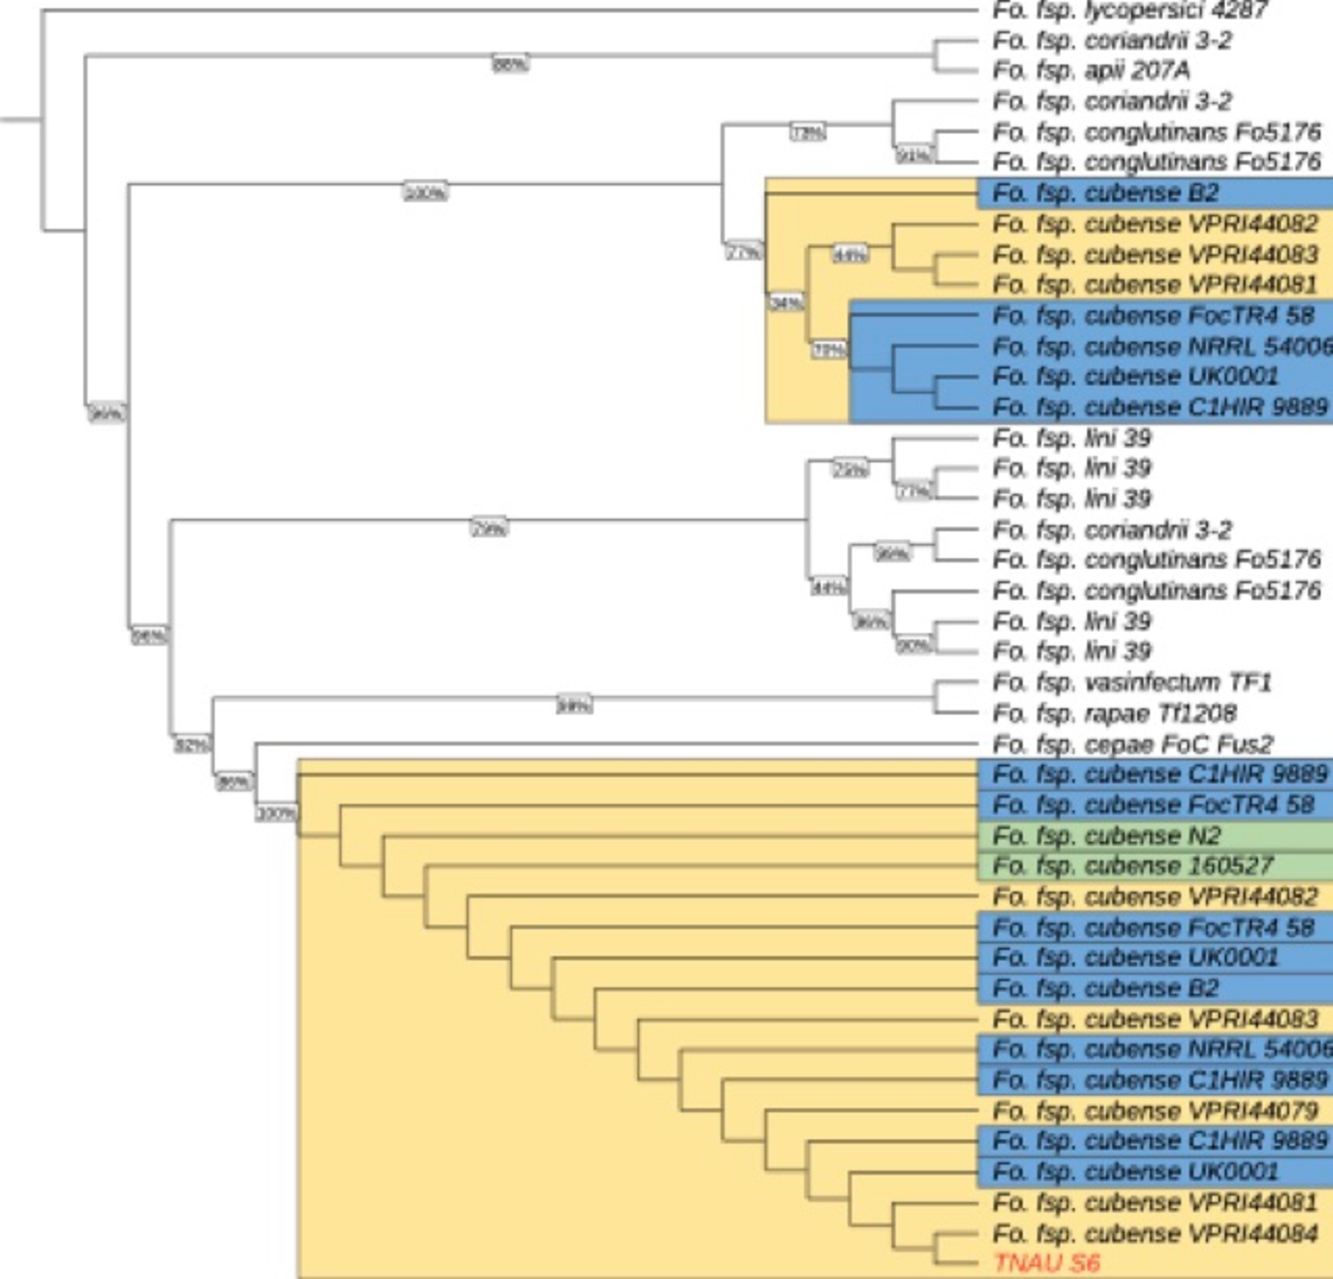
\includegraphics[]{Figures/FusSIX9-trimmed.phylo.pdf}
  \caption[\textit{SIX9} phylogeny of \textit{Fusarium} assemblies]{\textbf{\textit{SIX9} phylogeny of \textit{Fusarium} assemblies reveals \acl{Focub4} \textit{SIX9} homolog in S6}. \acl{sixg} identified using TBLASTN (cut off 1\-e\textsuperscript{6}) using \textit{SIX} genes from \acl{Foly} as a reference. \textit{SIX9} sequences from \ac{tnau} are shown in red text. \Acl{Focub1} \textit{SIX9} sequences are shown in green. \acl{Focub} \textit{SIX9} sequences with race not recorded are shown in yellow. Percentages represent values from 1,000 bootstrap replicates. The tree is rooted through \textit{F. oxysporum f. sp. lycopersici} \textit{SIX9}.}
  \label{fig:FusSIX9}
\end{figure}

\begin{figure}[htp!]
  \centering
  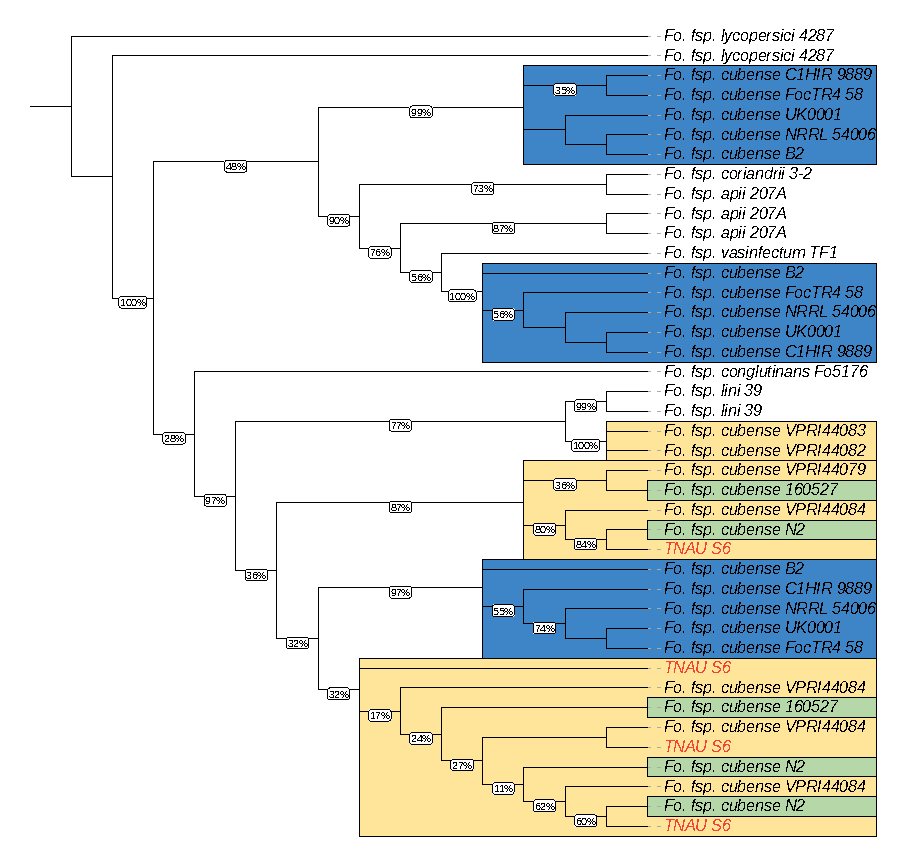
\includegraphics[]{Figures/FusSIX1.phylo.pdf}
  \caption[\textit{SIX1} phylogeny of \textit{Fusarium} assemblies]{\textbf{\textit{SIX1} phylogeny of \textit{Fusarium} assemblies}. \acl{sixg} identified using TBLASTN (cut off 1\-e\textsuperscript{6}) using \textit{SIX} genes from \acl{Foly} as a reference. \textit{SIX1} sequences from \ac{tnau} are shown in red text. \Acl{Focub1} \textit{SIX1} sequences are shown in green. \acl{Focub} \textit{SIX1} sequences with race not recorded are shown in yellow. Percentages represent values from 1,000 bootstrap replicates. The tree is rooted through \textit{F. oxysporum f. sp. lycopersici} \textit{SIX1}.}
  \label{fig:FusSIX1}
\end{figure}

\begin{figure}[hp!]
\centering
    \begin{subfigure}[]{0.9\textwidth}
        \centering
        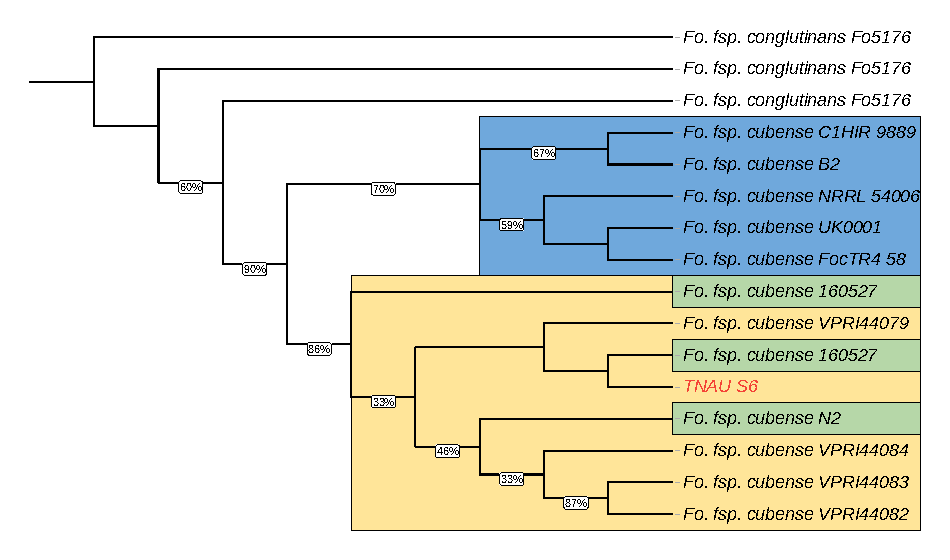
\includegraphics[width=\textwidth]{Figures/FusSIX4.phylo.pdf}
        \caption{}
        \label{fig:FusSIX4.phylo}
    \end{subfigure}
        \begin{subfigure}[]{0.9\textwidth}
        \centering
        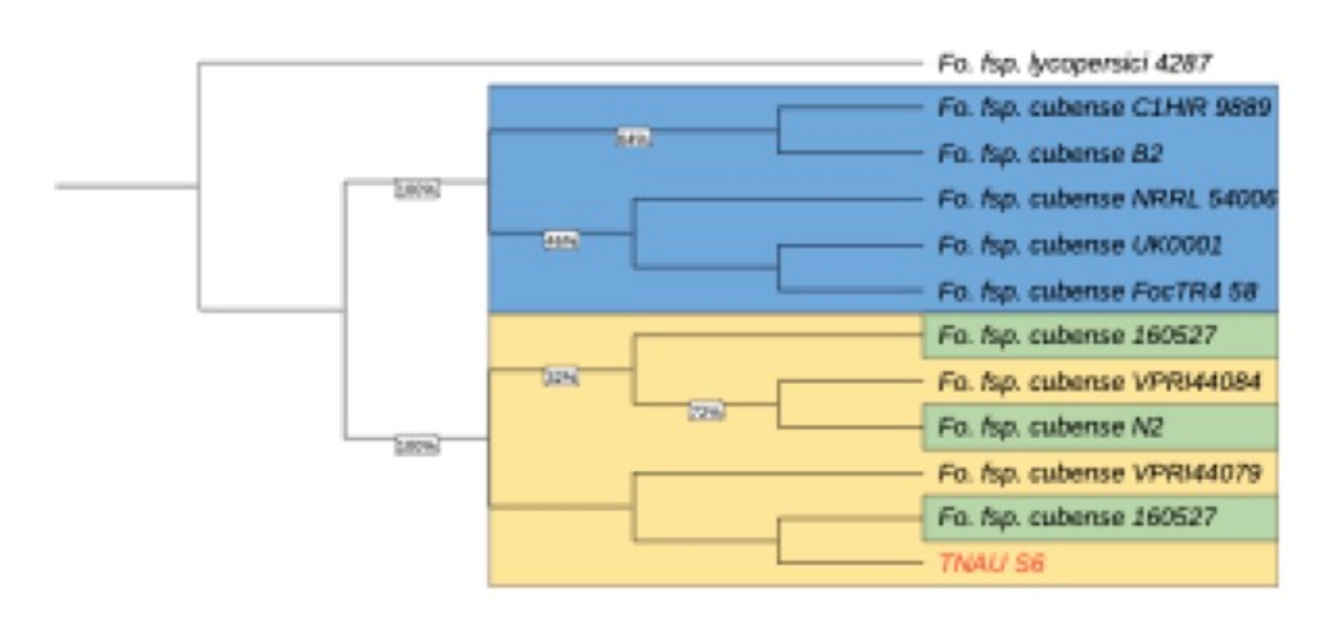
\includegraphics[width=\textwidth]{Figures/FusSIX6.phylo.pdf}
        \caption{}
        \label{fig:FusSIX6.phylo}
    \end{subfigure}
    \caption[\textit{SIX}6 gene phylogeny of \textit{Fusarium} assemblies]{\textbf{\textit{SIX} phylogeny of \textit{Fusarium} assemblies}.
    \acl{sixg} identified using TBLASTN (cut off 1\-e\textsuperscript{6}) using \textit{SIX} genes from \acl{Foly} as a reference. \textit{SIX6} sequences from \ac{tnau} are shown in red text.\Acl{Focub4} \textit{SIX6} sequences are in blue. \Acl{Focub1} \textit{SIX6} sequences are shown in green. \acl{Focub} \textit{SIX6} sequences with race not recorded are shown in yellow. Percentages represent values from 1,000 bootstrap replicates. \subref{fig:FusSIX4.phylo}) \textit{SIX4}. The tree is rooted through \textit{F. oxysporum f. sp. conglutinans} \textit{SIX4}. \subref{fig:FusSIX6.phylo}) \textit{SIX6}. The tree is rooted through \textit{F. oxysporum f. sp. lycopersici} \textit{SIX6}.}
    \label{fig:FusSIXMultiPhylo}
\end{figure}

\begin{figure}[htp!]
  \centering
  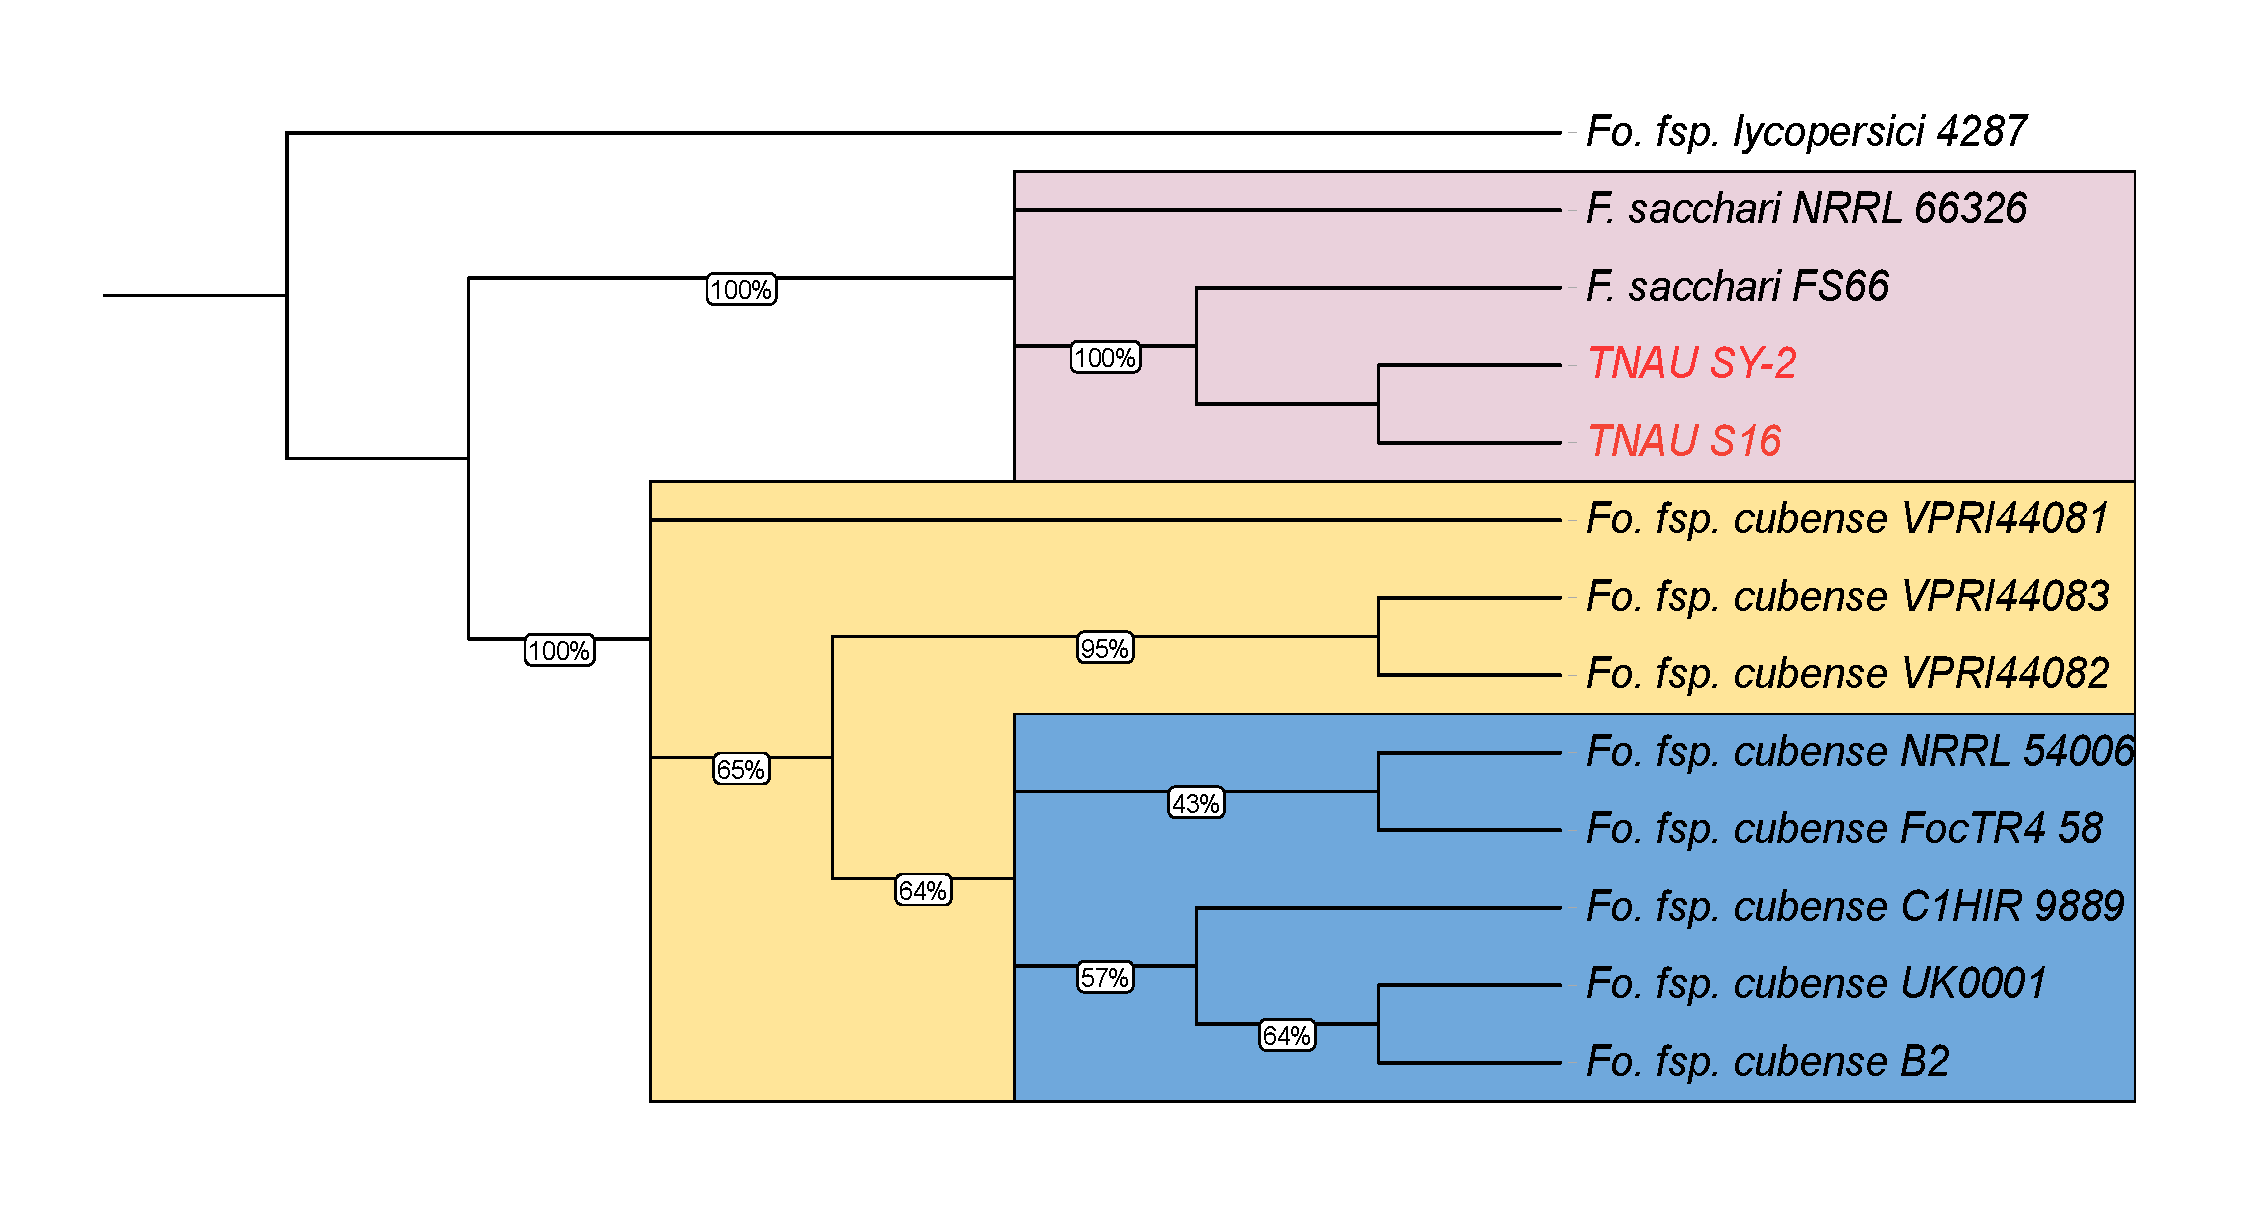
\includegraphics[width=15cm]{Figures/FusSIX2.Phylo.edited.pdf}
  \caption[\textit{SIX2} phylogeny of \textit{Fusarium} assemblies]{\textbf{\textit{SIX2} phylogeny of \textit{Fusarium} assemblies}. \acl{sixg} identified using TBLASTN (cut off 1\-e\textsuperscript{6}) using \textit{SIX} genes from \acl{Foly} as a reference. \textit{SIX2} sequences from \ac{tnau} are shown in red text. The \acl{Fs} clade is shown in pink. \Acl{Focub1} \textit{SIX2} sequences are shown in green. \acl{Focub} \textit{SIX2} sequences with race not recorded are shown in yellow. Percentages represent values from 1,000 bootstrap replicates. The tree is rooted through \textit{F. oxysporum} f. sp. \textit{lycopersici} \textit{SIX2}.}
  \label{fig:FusSIX2}
\end{figure}

\subsubsection{\ac{ce} distribution in Tamil Nadu Agricultural University \textit{Fusarium} genome assemblies.}
\label{tnauCEs}

Small secreted proteins (>30aa to <450aa)  from the predicted proteomes of the \ac{tnau} genome assemblies were analysed using EffectorP (v2.0.1) to identify potential effectors. Among the genome assemblies, S6 displayed the largest \acl{ce}ome, with 333 putative effectors, followed by genome assembly S32 with 314 \acp{ce}, while both SY-2 and S16 had 289 \acp{ce} each. Of these candidates, 132 were conserved between all genome assemblies when clustered at 80\% identity (Figure \ref{fig:TNAUVenn}). S6 also had the largest number of unique candidates when clustering at this percentage identity threshold, totalling 138. S32 had the next largest number of unique candidates, at 68. 70 of the candidates were shared between the S16 and SY-2 genome assemblies, but not the other genome assemblies. A total of 69 candidates were shared between S16, S32, and SY-2 but not in S6, and 39 candidates were shared between S6 and S32 but were not identified in SY-2 or S16 at the  80\% identity threshold. 

\begin{figure}[h!]
  \centering
  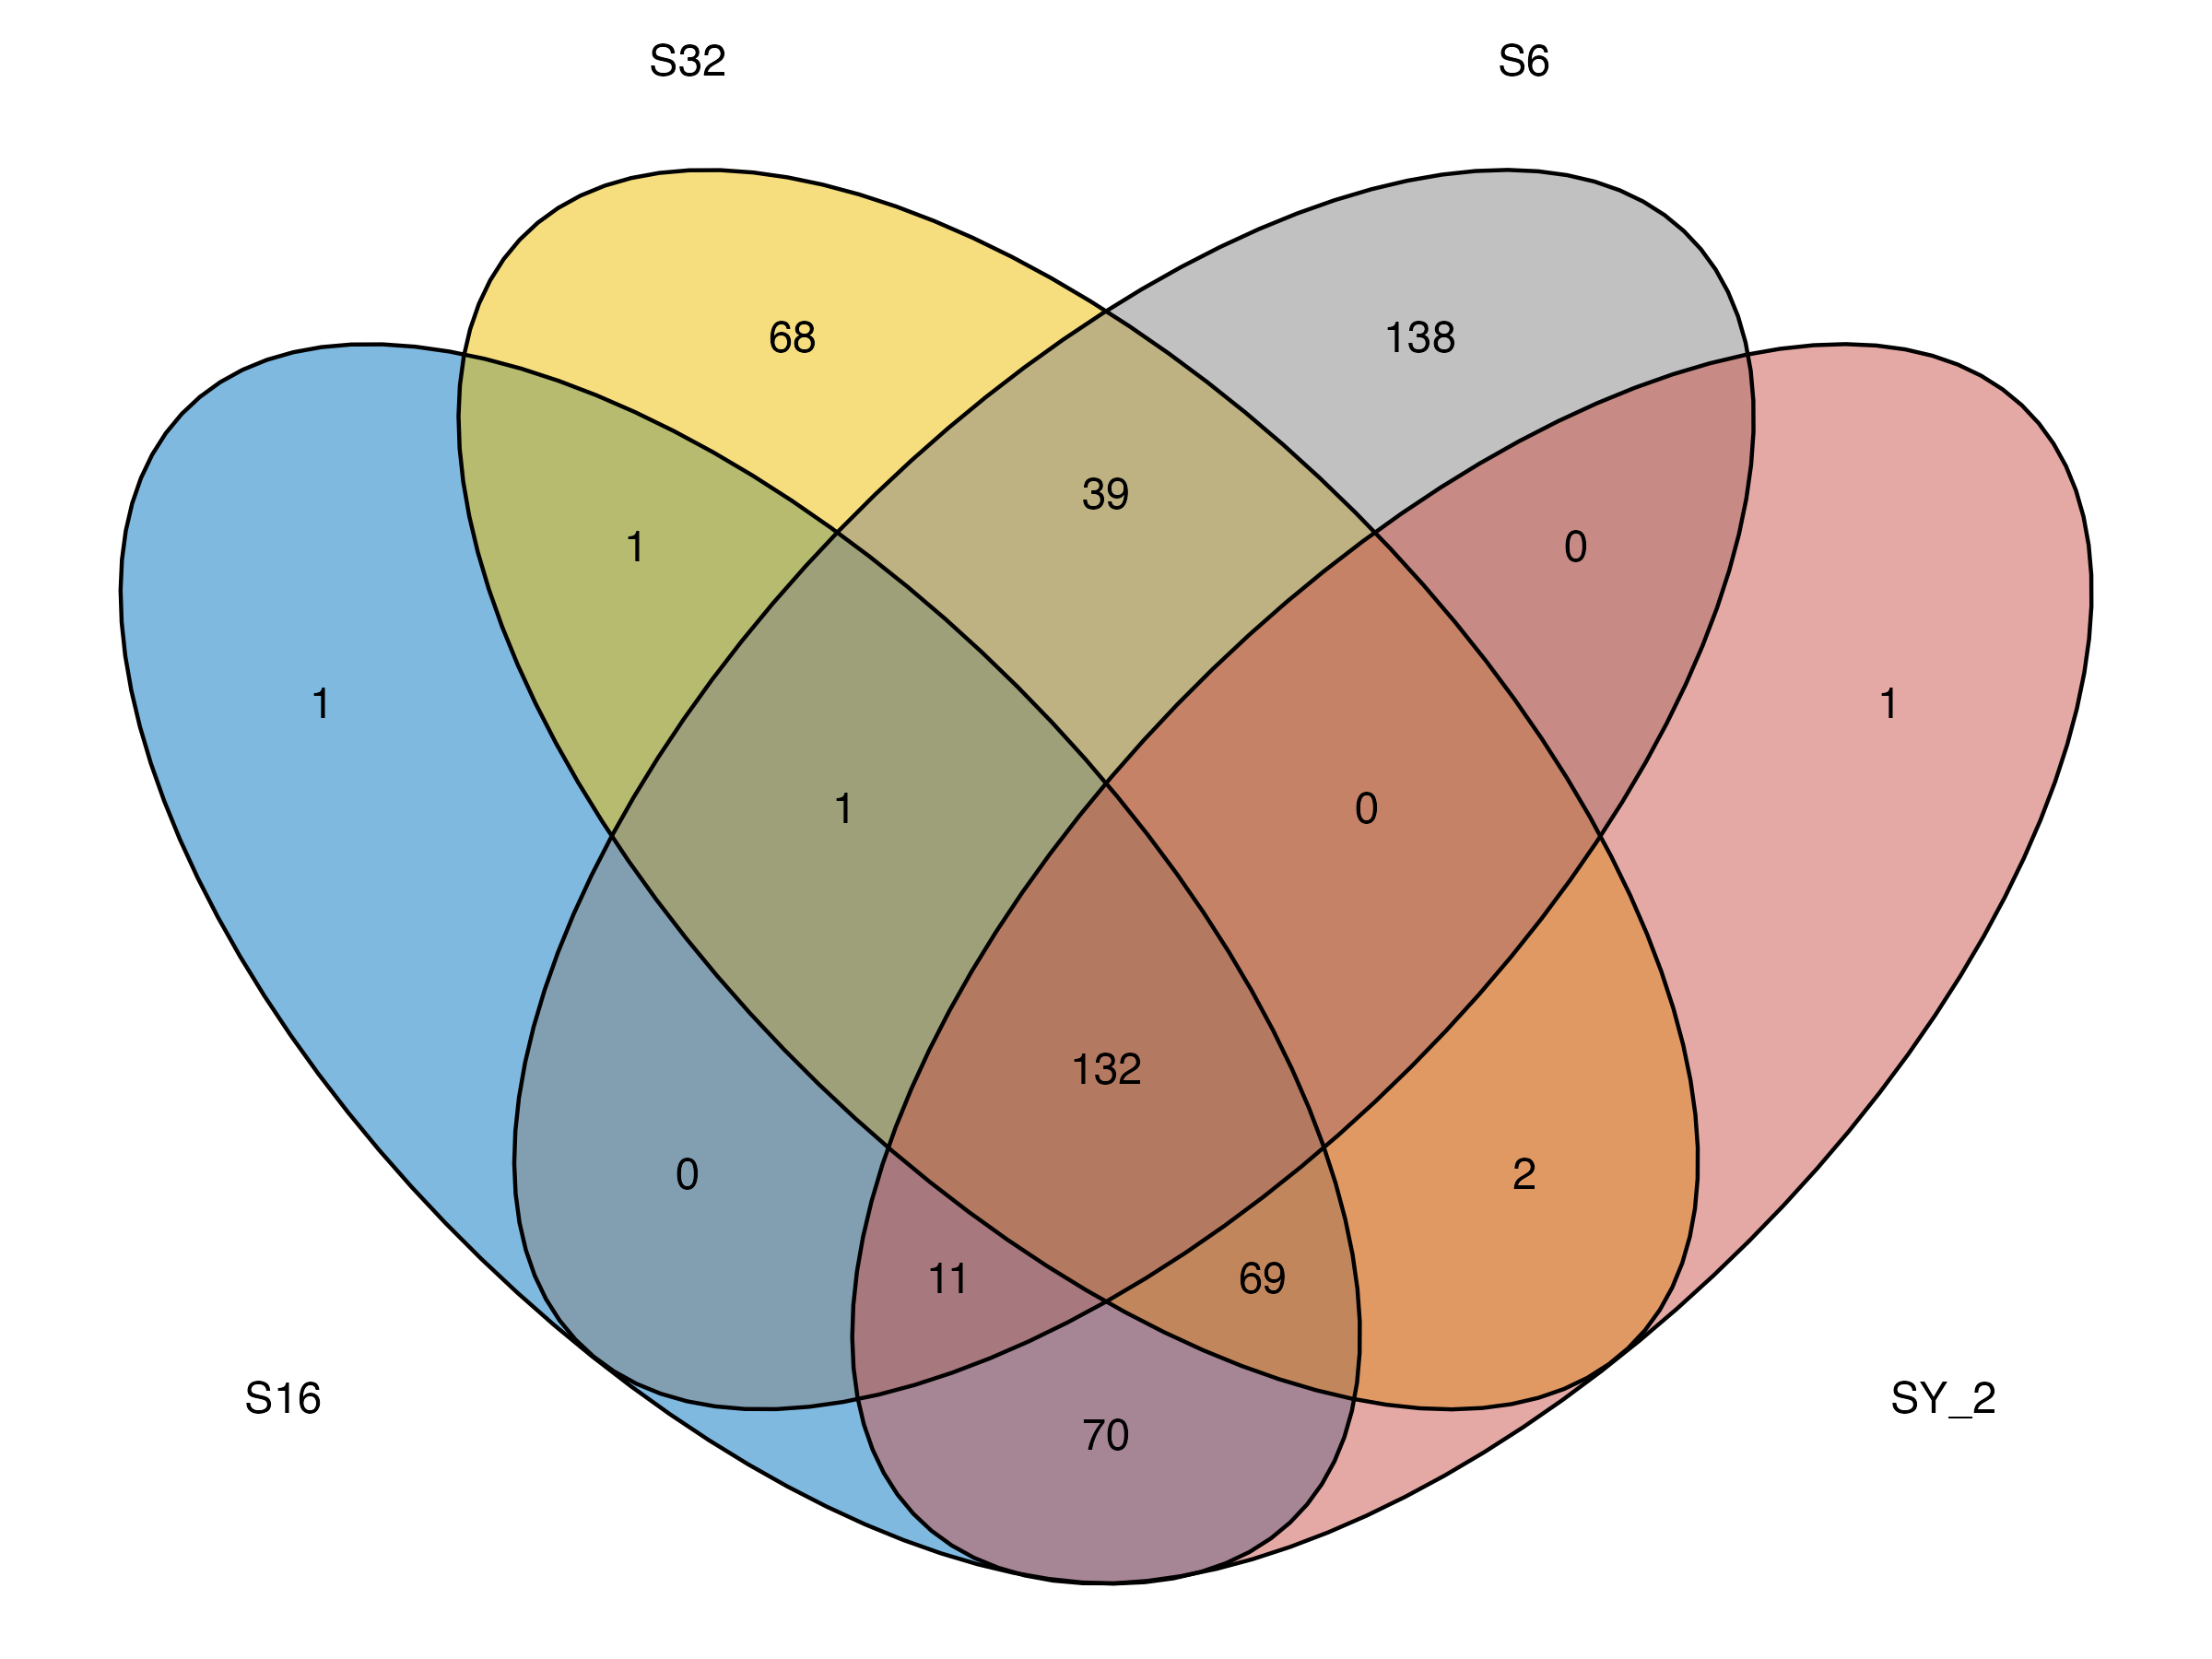
\includegraphics[width=12cm]{Figures/sharedCandEffsVenn.png}
  \caption[Distribution of \acp{ce} among Tamil Nadu Agricultural University \textit{Fusarium} genome assemblies.]{\textbf{Distribution of \acp{ce} among Tamil Nadu Agricultural University \textit{Fusarium} genome assemblies.} Numbers represent the total \acp{ce}. SY-2=red oval, S6=grey oval, S16=blue oval, S32=yellow oval.}
  \label{fig:TNAUVenn}
\end{figure}


%%%%%%%%%%%%%%%%%%%%%%%%%%%%%%%%%%%%%%%%%%%%%
%DISCUSSION
%%%%%%%%%%%%%%%%%%%%%%%%%%%%%%%%%%%%%%%%%%%%%
\newpage
\section{Discussion and Conclusions}

Collaborators at \ac{tnau}  investigated \ac{Focub} diversity in Tamil Nadu. They surveyed banana-growing areas, collecting samples from symptomatic banana, including the Cavendish variety, 'Grande Naine'. Of the isolates collected, SY-2, S6, S16, and S32 were chosen for further study due to their highly virulent phenotype on Cavendish banana. Collaborators report that DNA analysis confirmed SY-2, S6, S16, and S32 identity as \ac{Focub4} isolates. However, our study does not support their conclusions. Genomic analysis suggests that banana-pathogenic isolate S32 belongs to a clade within genus \textit{Fusarium} species that may represent an as-yet undescribed species , that S6 belongs to a clade usually associated with \ac{Focub1}, but   has acquired a \ac{Focub4} phenotype. Isolates SY-2 and S16 appear to belong to \ac{Fs}, a species  previously reported to be potentially pathogenic towards banana, having acquired genes from Fusarium oxysporum.

Initially, the raw read data supplied by collaborators at \ac{tnau} were aligned to high-quality \ac{Focub4} (\href{https://www.ncbi.nlm.nih.gov/datasets/genome/GCA_007994515.1/}{GCA\_007994515.1}) and \ac{Focub1} (\href{https://www.ncbi.nlm.nih.gov/datasets/genome/GCA_005930515.1/}{GCA\_005930515.1})  assemblies for a reference-guided assembly approach. However, alignment rates and web BLASTN searches of the unmapped reads against the nr/nt database contradicted TNAU's initial classifications, and revealed bacterial contamination in the S6 and S32 datasets\footnote{Later supported by BlobTools (v1.1.1) analysis of \textit{de novo} assembly constructed using all raw reads (See section: \ref{sec:BlobToolsOfS6S32-allreads}).}. Consequently, raw reads were  mapped to assemblies for which a large number of highly similar ($ \geq90\% $ identity) BLASTN hits were identified. Genome assemblies for SY-2, S16, and S32 showed closer alignment to the \textit{F. sacchari} reference compared to the \ac{Focub} references, and S6 and S32 contained contamination from \textit{S. maltophilia}. 

As these results suggested that SY-2, S16, and S32 are not \ac{Focub4} isolates, it was no longer clear which species should be used as a reference for a reference-guided assembly. Further, the \ac{tnau} isolates displayed a highly virulent phenotype and a reference-guided assembly could lose any large-scale rearrangements in the genome which may contribute to this phenotype. However, contamination in the S6 and S32 data meant that a \textit{de novo} genome assembly for these isolates is likely to result in misassembled contigs that are chimeric part target species, part non-target species). These contigs can be challenging to identify and may result in contigs that should remain in the assembly being filtered out, and contigs that do not belong to the target species being kept in the assembly, even when using BlobTools (v1.1.1.) to separate target and non-target contigs \parencite{Cornet2022}, so must be removed from the raw read data. 

Consequently, genomes for SY-2 and S16 were assembled \textit{de novo} and S6 and S32 were assembled \textit{de novo} using only the reads that mapped to reference genomes with the highest mapping value. For S6, therefore, a \textit{de novo} genome assembly was generated using the raw reads which mapped to \ac{Focub1} 160527 (\href{https://www.ncbi.nlm.nih.gov/datasets/genome/GCA_005930515.1/}{GCA\_005930515.1}) reference and for S32 a \textit{de novo} assembly was generated using the raw reads which mapped to the \ac{Fs} FS66 (\href{https://www.ncbi.nlm.nih.gov/datasets/genome/GCA_017165645.1/}{GCA\_017165645.1}) reference. BlobTools (v1.1.1) was used to confirm that the levels of contamination in the assemblies had been reduced, pinpoint any potential contaminant contigs to remove, and support isolate classification. Predicted protein coding genes, percentage GC content, size, and \ac{busco} scores for the contaminant filtered assemblies were comparable to other \textit{Fusarium} short-read assemblies (see: \textcite{DitaHerai2013, Chiara2015, Srivastava2018}).

As the identity of \ac{tnau} isolates was uncertain, we queried the genetic markers \acf{tef} and \acf{rbp2} extracted from the assemblies against Fusariod-ID MSLT and \ac{ncbi} BLAST databases. For the S16 extracted \ac{tef}, the top hits in the Fusariod MSLT database and \ac{ncbi} database were associated with the \ac{FFSC} and \ac{Fs}, respectively (Table \ref{tab:Tef1-MLSTdb}, Table \ref{tab:Tef1-NCBIdb}). In the case of S6, the extracted \ac{tef} sequences indicated a potential association with \ac{FOSC}, although specific matches for \ac{Focub} \ac{tef} sequences were not among the top results from both databases. Notably, no matches were found for the S32 \ac{tef} sequences in the Fusarioid-ID MSLT database, while hits in the \ac{ncbi} GenBank database pointed towards \ac{Ff} sequences, further suggesting that SY-2, S16, and S32 were members of the \ac{FFSC} pathogenic towards banana and that S6 is a \ac{Fo} isolate. Expanding the marker count has the potential to fortify the robustness of our phylogenetic inferences. 

Phylogenies generated using the same genetic markers (\ac{tef} and \ac{rbp2}) supported these initial conclusions. S6 clustered within a \ac{Focub1} clade in both \acs{tef} and \ac{rbp2} phylogenies (Figure: \ref{fig:TEF1aPhylo}, Appendix \ref{fig:rbp2Phylo}) and, S16 appeared to align closely with SY-2 and reference \ac{Fs} species in the phylogenetic analysis. Notably, S32's placement suggested a relation to the recently proposed species, \textit{F. mindanaoense}, identified in symptomatic Cavendish bananas in the Philippines \parencite{Nozawa2023}. \textcite{Nozawa2023} suggest that \textit{F. mindanaoense} is a sister linage of the \ac{Fs}, which our data supports. The authors also suggest this newly proposed species has acquired the \ac{sixg} \textit{SIX6}, though they have not confirmed the \textit{SIX6} homolog identified is involved in virulence. Though S32 falls within the same clade as the novel species proposed by \textcite{Nozawa2023}, we did not identify a \textit{SIX6} homolog in the S32 assembly, which suggests that alternative virulence genes are associated with S32 pathogenicity in banana. 

The absence of any \acp{sixg} in S32 distinguishes it from the other \ac{tnau} genome assemblies which also appear to be in the \ac{FFSC}, as SY-2 and S16 both contain a \textit{SIX2} homologue. Further, the \textit{SIX2} homologue identified in the SY-2 and S16 assemblies supports their classification as \ac{Fs} isolates pathogenic towards banana, as they fall within the same clade as the \ac{Fs} isolates included, FS66 and NRRL 66326. FS66 is reported as pathogenic towards banana \parencite{Cui2021}, and the FS66, SY-2, and S16 \textit{SIX2} homologues have 100\% identity. However, the role of the \textit{SIX2} homolog in \ac{Fs} has not yet been characterised. The presence of \textit{SIX2} in S16 and SY-2 genomes may contribute towards their virulence in Cavendish banana varieties, as \textit{SIX2} is only found in \ac{r4} genomes of \ac{Focub} \parencite{Czislowski2018}. However, \textcite{An2019} suggest that \textit{SIX2} has a reduced role in virulence as inoculation of \textit{Musa acuminata} L. AAA group, ‘Brazilian’ plantlets. \textit{SIX2} knock-out mutants showed similar disease progress as plants inoculated with wild-type \ac{Focub4}. Also, confirmation of \textit{SIX2} expression during infection in SY-2 or S16 is still required. 

Variation in \acp{sixg} in S6 compared to other \ac{Focub} genome assemblies can also be observed. The \acp{sixg} identified in S6 consistently fell within the same clade as \ac{Focub1} genomes, though copy number varied. It is important to consider the assembly approach, however. Despite using raw reads that mapped to the \ac{Focub1} assembly from \textcite{Asai2019} (\href{https://www.ncbi.nlm.nih.gov/datasets/genome/GCA_005930515.1/}{GCA\_005930515.1}) or had no-hit, the S6 genome was assembled \textit{de novo}. This approach aimed to ensure an unbiased depiction of the genetic structure, including the \acp{sixg} sequence, in the S6 (and S32) assembly. Interestingly, collaborators at \ac{tnau} suggest that S6 is highly virulent towards Cavendish banana varieties. It is of note, that a \textit{SIX13} homolog was identified in the other \ac{Focub1} genomes used in this study, but was not found in the S6 assembly.  This may be due to the assembly quality of S6. High contiguity is often challenging to achieve in repeat-rich regions of short-read assemblies \parencite{Treangen2012, Peona2021}, which is where the many \textit{Fusarium} effectors can be found \parencite{Ma2010, Schmidt2013, Armitage2018}. It is possible that no \textit{SIX13} was identified due to genome assembly fragmentation. Alternatively, the absence of \textit{SIX13} may contribute towards S6 virulence on Cavendish banana. 

As well as \acp{sixg}, other \acp{ce} were identified and clustered based on sequence identity. Though this chapter does not explore these \acp{ce} in-depth, similarities can be identified which help to support our classification of the \ac{tnau} isolates. The \ac{ce} profiles of SY-2 and S16 reinforce the proposition that these two isolates are closely related if not isolates of the same \ac{Fs} strain. Both SY-2 and S16 had 289 \acp{ce} each, 282 of which are shared when clustering at 80\% identity, and only one candidate was unique to each genome assembly. For S6, however, 138 of its 333 \acp{ce} were not shared between any of the other \ac{tnau} genome assemblies. Comparison of these predicted effectors against the effector repertoires of \ac{Focub} and \ac{Fs} would help to further corroborate our classification of the \ac{tnau} isolates, and may provide insights into the \textit{Fusarium} host specificity. It is important to highlight, however, that it may be challenging to conclude from downstream analyses on the predicted proteomes of the \ac{tnau} genome assemblies. Annotations were generated without transcriptome data from these genome assemblies, and assemblies may contain fragments of contamination although much care was taken to filter contaminants from the raw data. Further, assemblies are not highly contiguous ($ \geq408\% $ contigs), so gene models may become truncated or missed, particularly genes typically found in repeat-rich regions. 

\textcite{Thangavelu2020} recently described \ac{Focub1} isolates in the 0125 and 01220 \ac{vcg} complex, found in Tamil Nadu, that are pathogenic towards Cavendish banana. It is possible that S6 belongs to this \ac{vcg} complex. Laboratory assays for determining \ac{vcg} are required for S6. I recognise that the classification of S6 as \ac{Focub1} isolate that is pathogenic towards a Cavendish variety is conflicting, as \ac{Focub} race is determined by host specificity. \textcite{Torres2021} argue that race classification be used as a "phenotypic rather than taxonomic designation", but in this instance, it does not highlight the diversity of \textit{Fusarium} in the region, so S6 has been described as an \ac{Focub1} isolate displaying a \ac{Focub4} phenotype.

The spread of \ac{Focub} throughout banana-growing regions is of major concern, particularly in India. Currently, much emphasis is placed on the threat of \ac{Focub4} to Cavendish production in this region \parencite{Viljoen2020, Damodaran2019}, but our results suggest that the \ac{Focub4} \ac{vcg} 01213/16 is not the only threat. All isolates assessed in this study are reported to be highly virulent on Cavendish banana by collaborators; S6 appears to be a \ac{Focub1} isolate displaying a \ac{Focub4} phenotype and SY-2, S16, and S32 are part of the \ac{FFSC}. As the FS66 isolate was identified in China, and novel species described by \textcite{Nozawa2023} were identified in the Philippines, it is possible that these strains can be found in other banana regions in India, and also poses a threat for introduction to other banana-growing countries. The discovery of potentially novel causal agents of \ac{fwb} in the region means it is imperative that \ac{fwb} continue to be monitored, and that accurate diagnostics and effective controls are studied and employed.  
